COMSOL Multiphysics\textsuperscript{TM} is a comprehensive software suite for finite element analysis, solving, and simulation across a wide array of physics and engineering disciplines, particularly focusing on coupled phenomena and multiphysics interactions. It enables the creation and simulation of physics-based models and applications in an intuitive, interactive workspace.

COMSOL software supports a broad spectrum of applications, from electromagnetics and structural mechanics to acoustics, fluid dynamics, heat transfer, and chemical engineering. COMSOL features an extensive array of modules, including the Wave Optics module for optical applications simulations like wave propagation in fiber optics and photonics, the Semiconductor module for the analysis of semiconductor devices such as diodes and transistors, and the AC/DC module for examining electric and magnetic fields in static and low-frequency scenarios. For my thesis, which involves analyzing ray paths in optical systems, I will be utilizing the Ray Optics module.

% ----- THE MODELLING WORKFLOW -----
\section{The COMSOL Modelling Workflow}
Briefly the modelling workflow consists of the following steps, if you start a model completely from scratch:

\begin{enumerate}
    \item \textbf{Initialization of the Model Environment}: Preparing the foundational settings for the simulation.
    \item \textbf{Geometry Construction}: Designing the model's physical layout.
    \item \textbf{Material Property Specification}: Assigning specific materials to the model components.
    \item \textbf{Physics Boundary Conditions Definition}: Establishing the physical constraints and conditions.
    \item \textbf{Mesh Generation}: Creating the computational grid over the model.
    \item \textbf{Simulation Execution}: Performing the actual computational analysis.
    \item \textbf{Results Post-Processing}: Analyzing and visualizing the simulation outcomes.
\end{enumerate}

In this context, I will demonstrate this workflow first through a simple project, illustrating COMSOL's robust capabilities and the straightforwardness of applying this workflow across various projects. It's important to recognize that this workflow remains consistent across different physics simulations, which will guide the development of subsequent models for my thesis.

This demonstration will focus on simulating Joule heating within a busbar, a process where electric current passing through metal results in heating due to electrical resistance.

The busbar in question will incorporate three titanium bolts, with electrical current flowing from a single bolt on one end to a pair of bolts at the opposite end. The objective is to observe the resulting temperature distribution as the busbar undergoes heating.

% Busbar image
\begin{figure}[ht!]
  \centering
  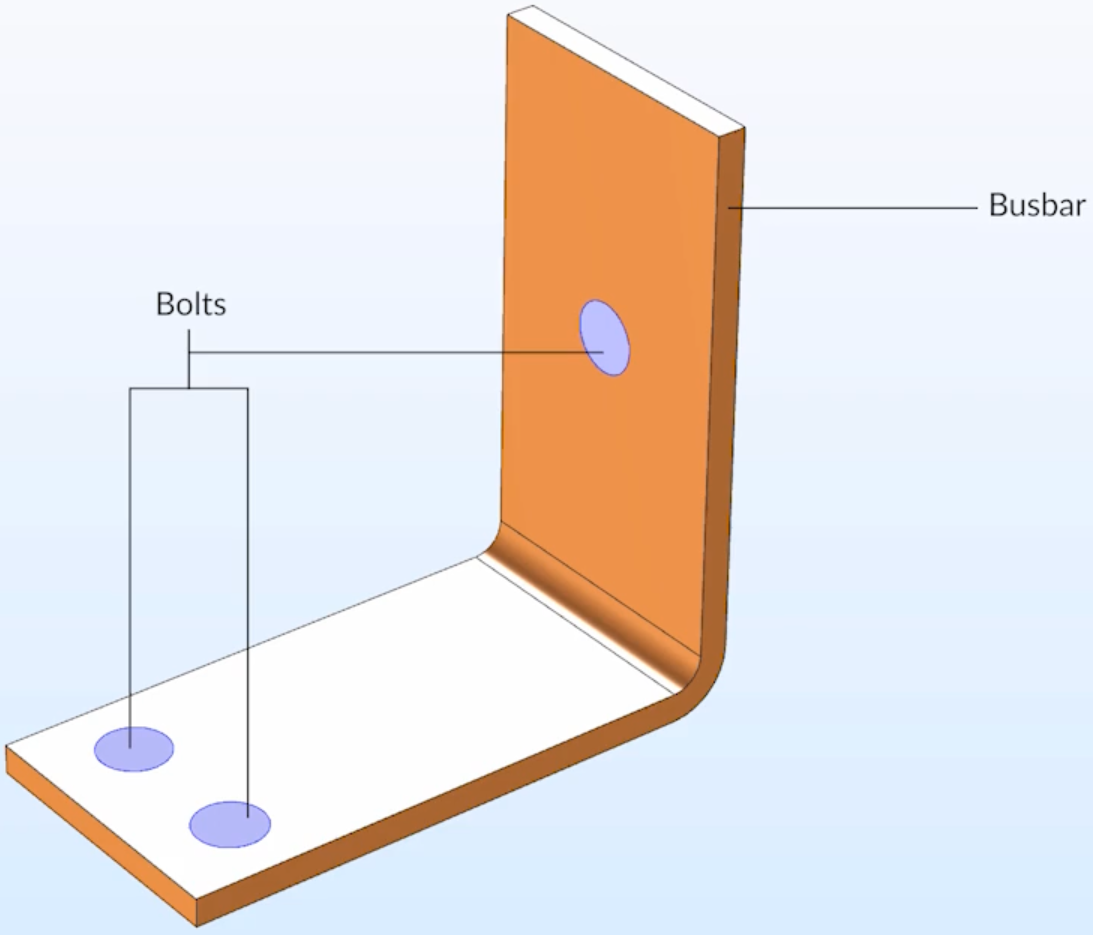
\includegraphics[width=0.4\textwidth]{Chapters/Figures/Chapter 3 Figures/Busbar.png}
  \caption{ Source: \cite{}}
  \label{}
\end{figure}

% SUBSECTION --- Setting up the model environment ---
\subsection{Setting Up the Model Environment}.
% TODO: Add set-up screen image
\begin{figure}[ht!]
  \centering
  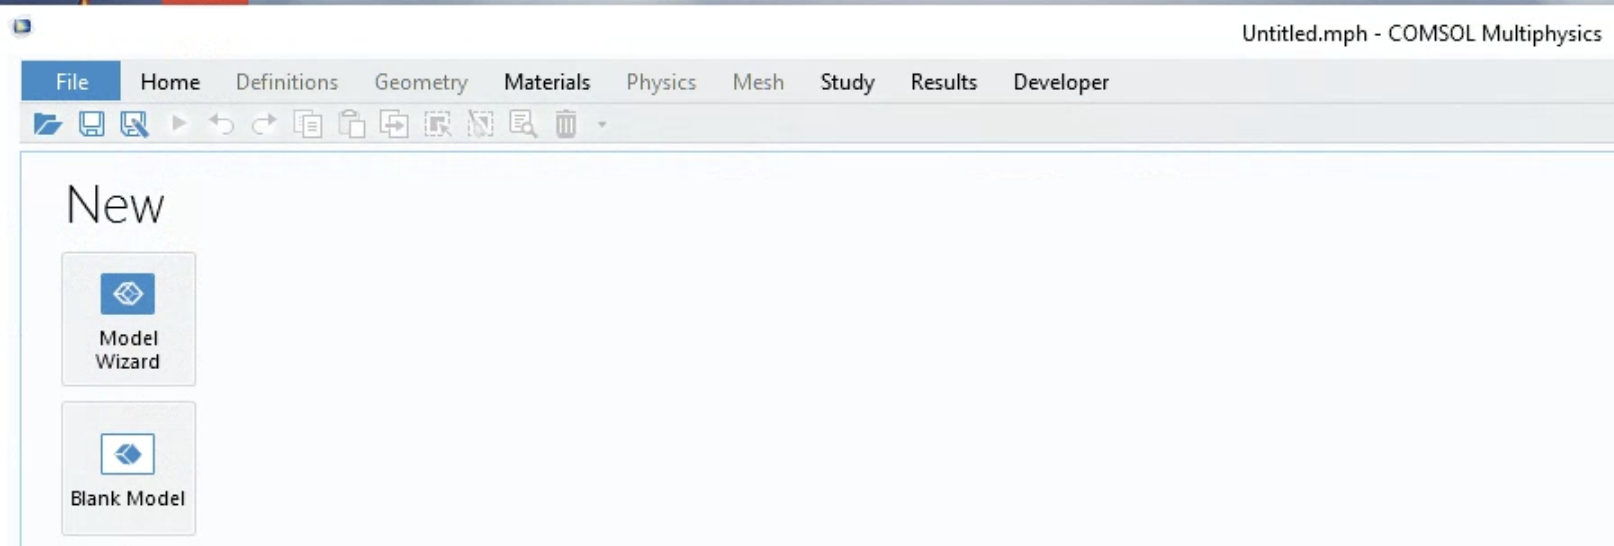
\includegraphics[width=0.4\textwidth]{Chapters/Figures/Chapter 3 Figures/Set-up Screen.png}
  \caption{ Source: \cite{}}
  \label{}
\end{figure}

Upon launching COMSOL, you are presented with an option to initiate a new project: selecting a Blank Model for starting anew or opting for the Model Wizard for a guided setup. The Model Wizard is advisable for its structured selection process integral to configuring your model. Conversely, choosing a Blank Model grants immediate access to the COMSOL desktop interface, bypassing the preliminary selections required by the Model Wizard.

% TODO: Add "Select Space Dimension" image
\begin{figure}[ht!]
  \centering
  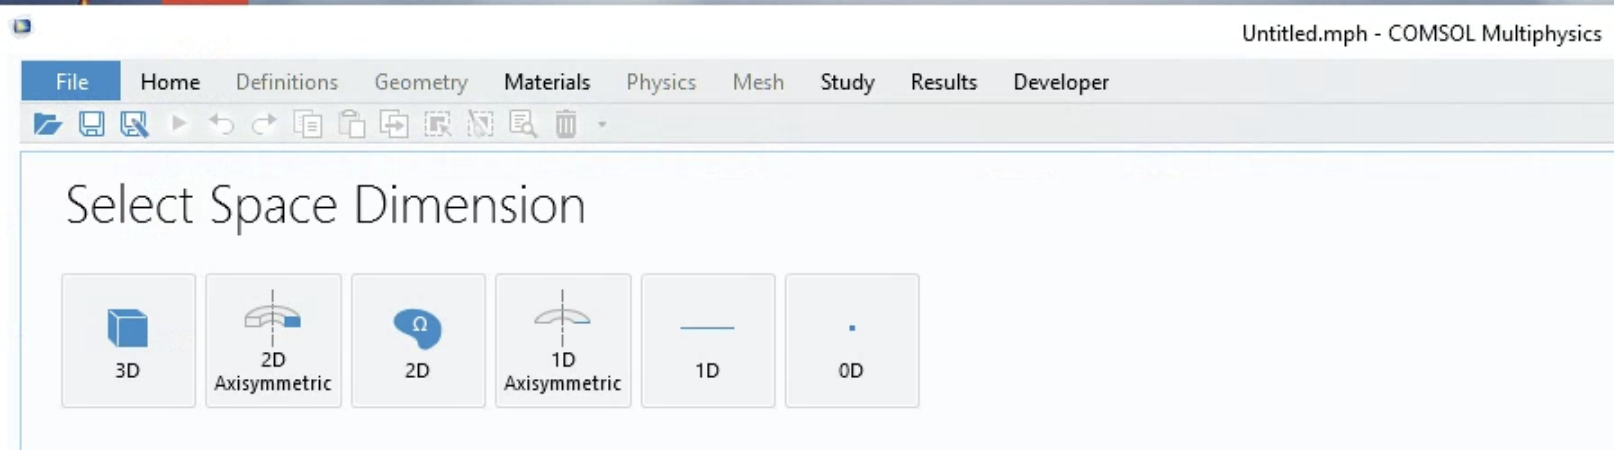
\includegraphics[width=0.4\textwidth]{Chapters/Figures/Chapter 3 Figures/Select Space Dimension.png}
  \caption{ Source: \cite{}}
  \label{}
\end{figure}

Since our busbar model requires a three-dimensional framework, we select the "3D" option.

% TODO: Add "Select Physics" image
\begin{figure}[ht!]
  \centering
  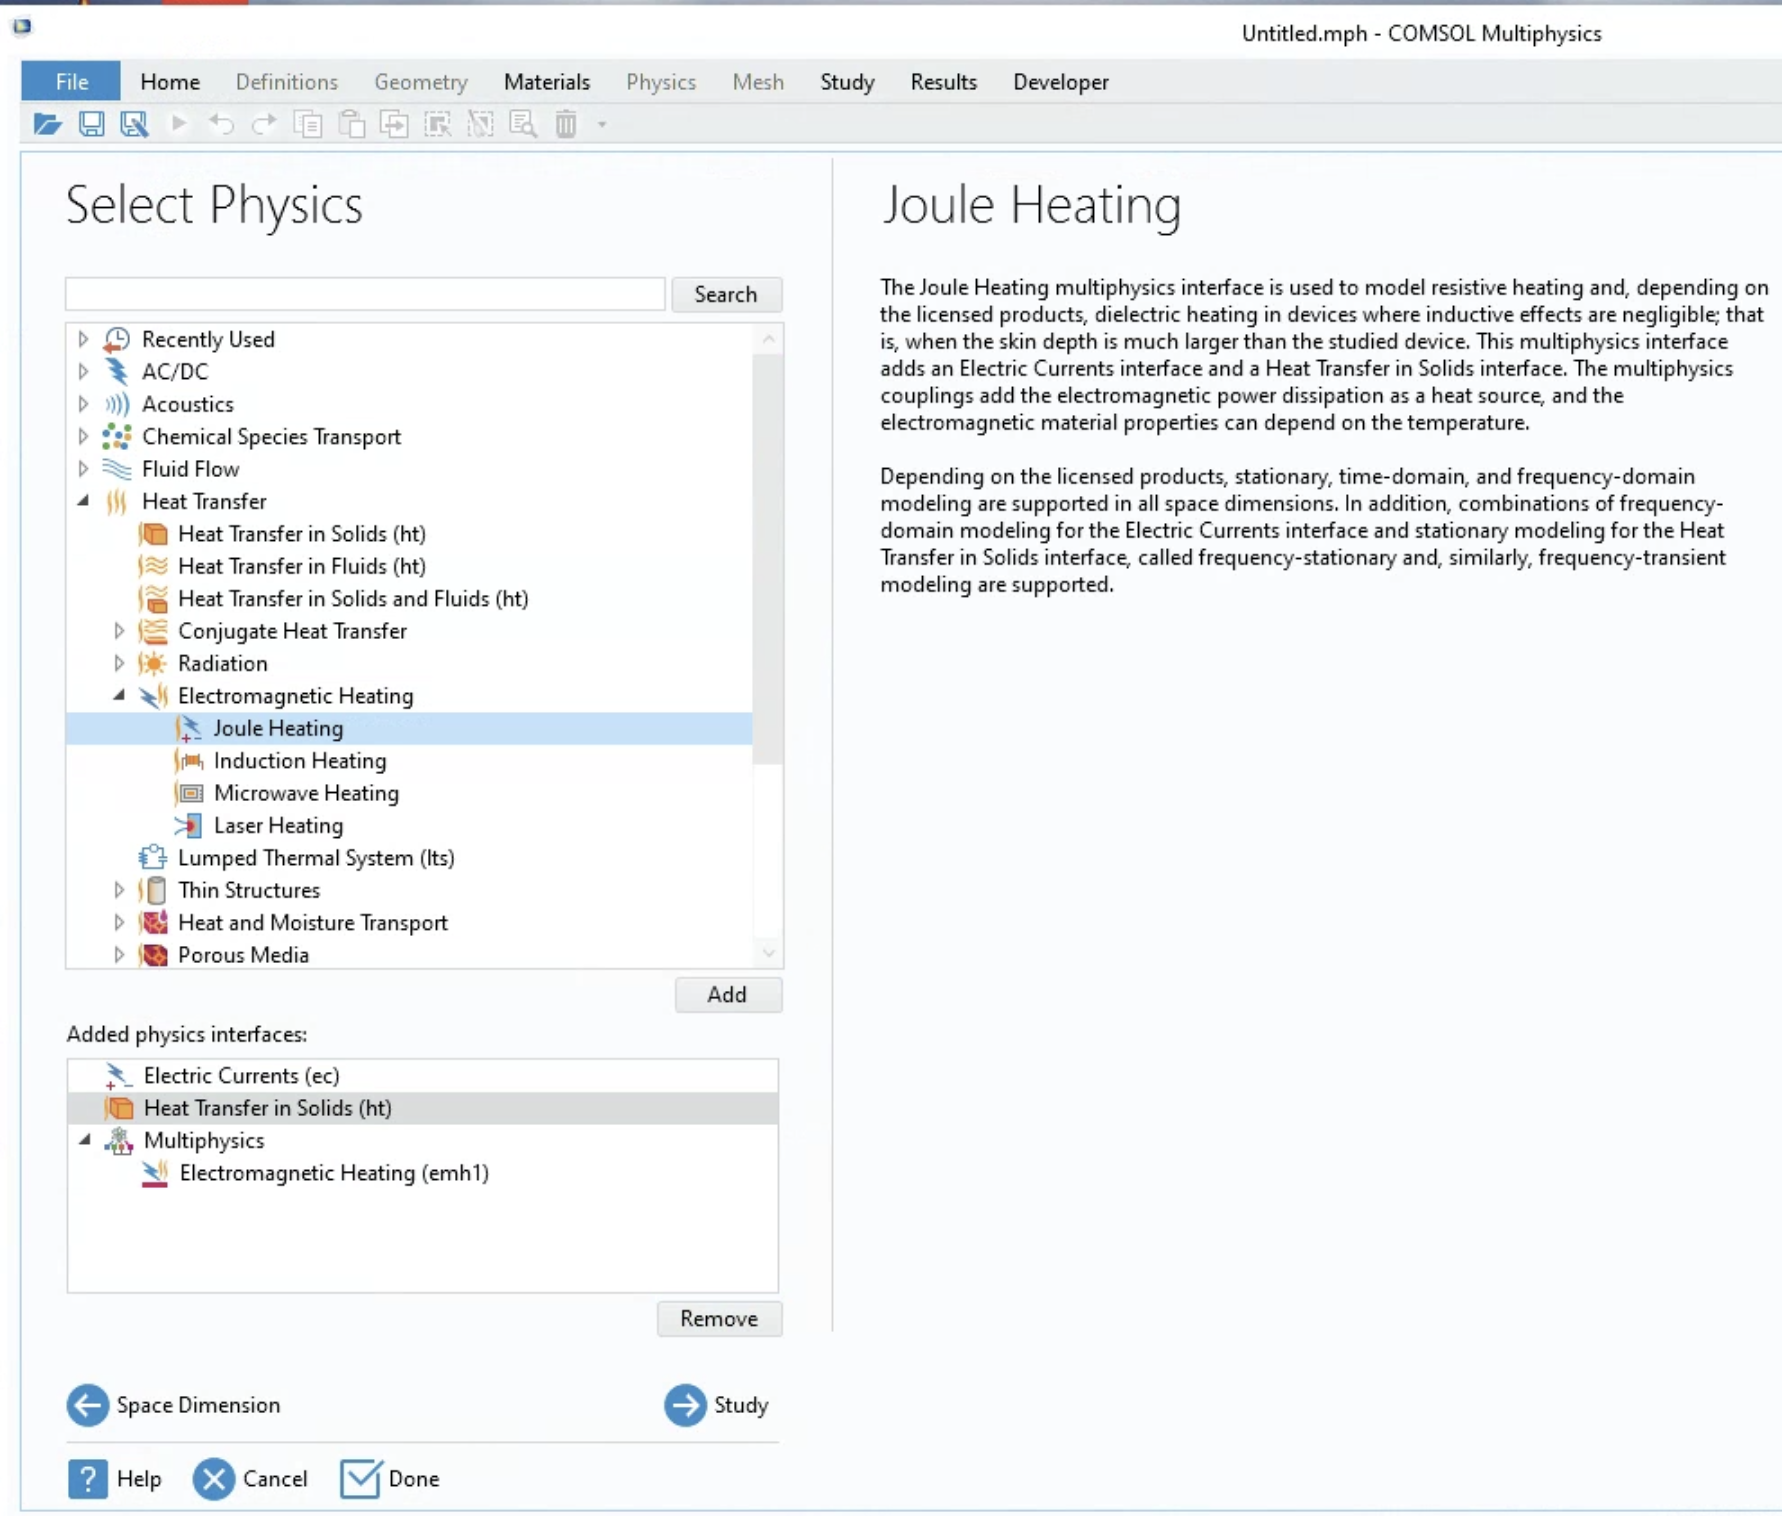
\includegraphics[width=0.4\textwidth]{Chapters/Figures/Chapter 3 Figures/Select Physics.png}
  \caption{ Source: \cite{}}
  \label{}
\end{figure}

Subsequently, we arrive at a prompt to select the desired physics for the model. In our case, we opt for Joule heating. In another scenario, for instance, if one's project was on thin-film fluid flow, navigating to the ``Fluid Flow'' node and selecting ``Thin-Film Flow'' would be the procedure. Adding ``Joule Heating'' automatically associates it with related physics categories like ``Electric Currents (ec)'' and ``Heat Transfer in Solids (ht),'' indicating that ``Joule Heating'' encompasses a composite interface with multiple physics elements integrated.

The selection of physics for exploration significantly hinges on the project's specific requirements and the level of access provided by your COMSOL subscription. For example, acquiring the ``Ray Optics'' module necessary for my thesis entailed a waiting period due to initial subscription limitations. Therefore, early verification of the required physics for your project is recommended.

To proceed, we select ``Study''.

% TODO: Add "Select Study" image
\begin{figure}[ht!]
  \centering
  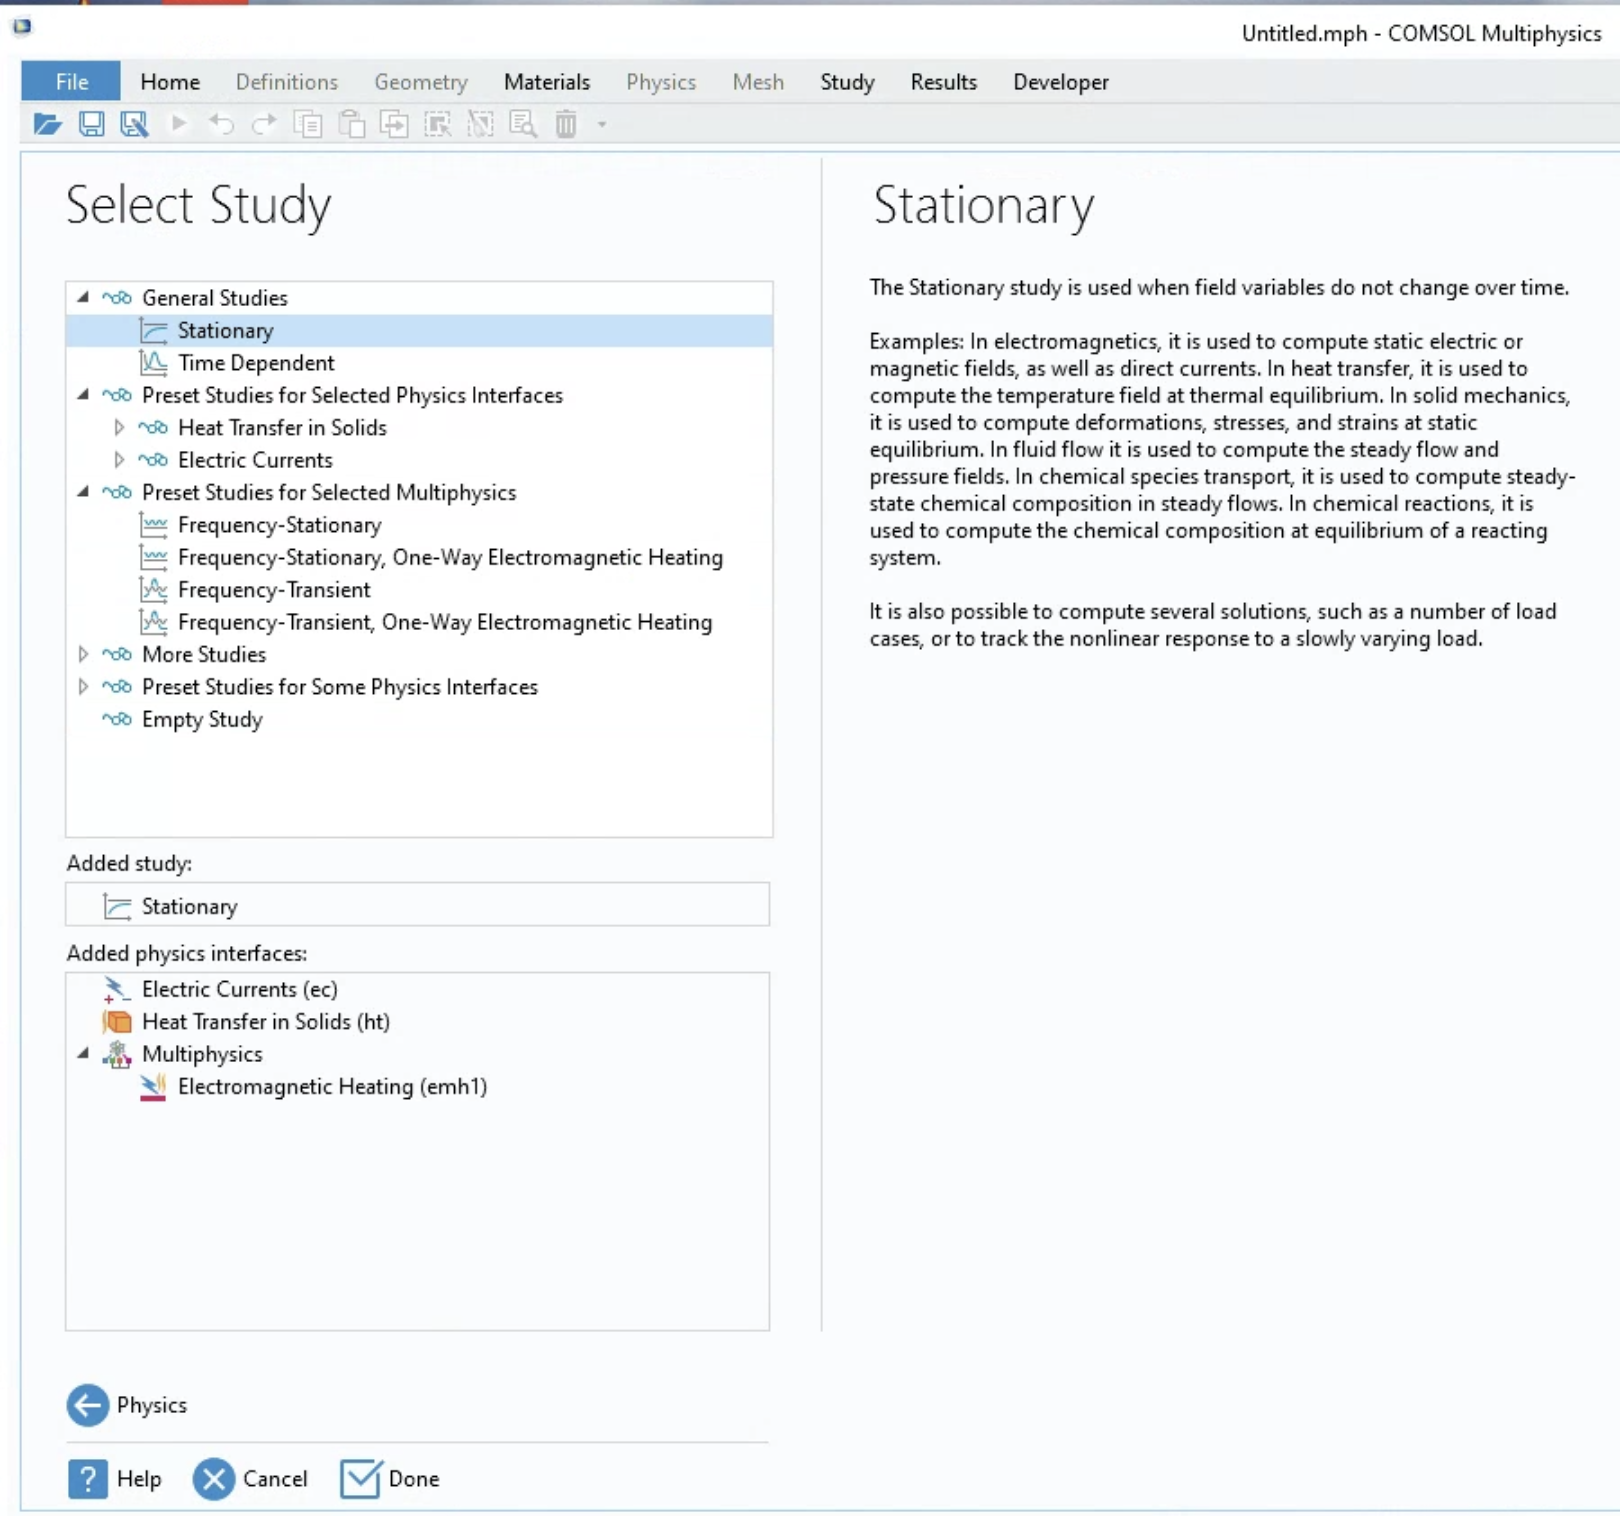
\includegraphics[width=0.4\textwidth]{Chapters/Figures/Chapter 3 Figures/Select Study.png}
  \caption{ Source: \cite{}}
  \label{}
\end{figure}

Upon accessing this interface, we are presented with an assortment of study options, determined by our earlier selections regarding the model's spatial dimensions and physics. For our busbar analysis, the ``Stationary'' study suffices, given its static nature. After selecting ``Done'', we transition to the COMSOL desktop environment.


% TODO: Add "COMSOL Desktop" image
\begin{figure}[ht!]
  \centering
  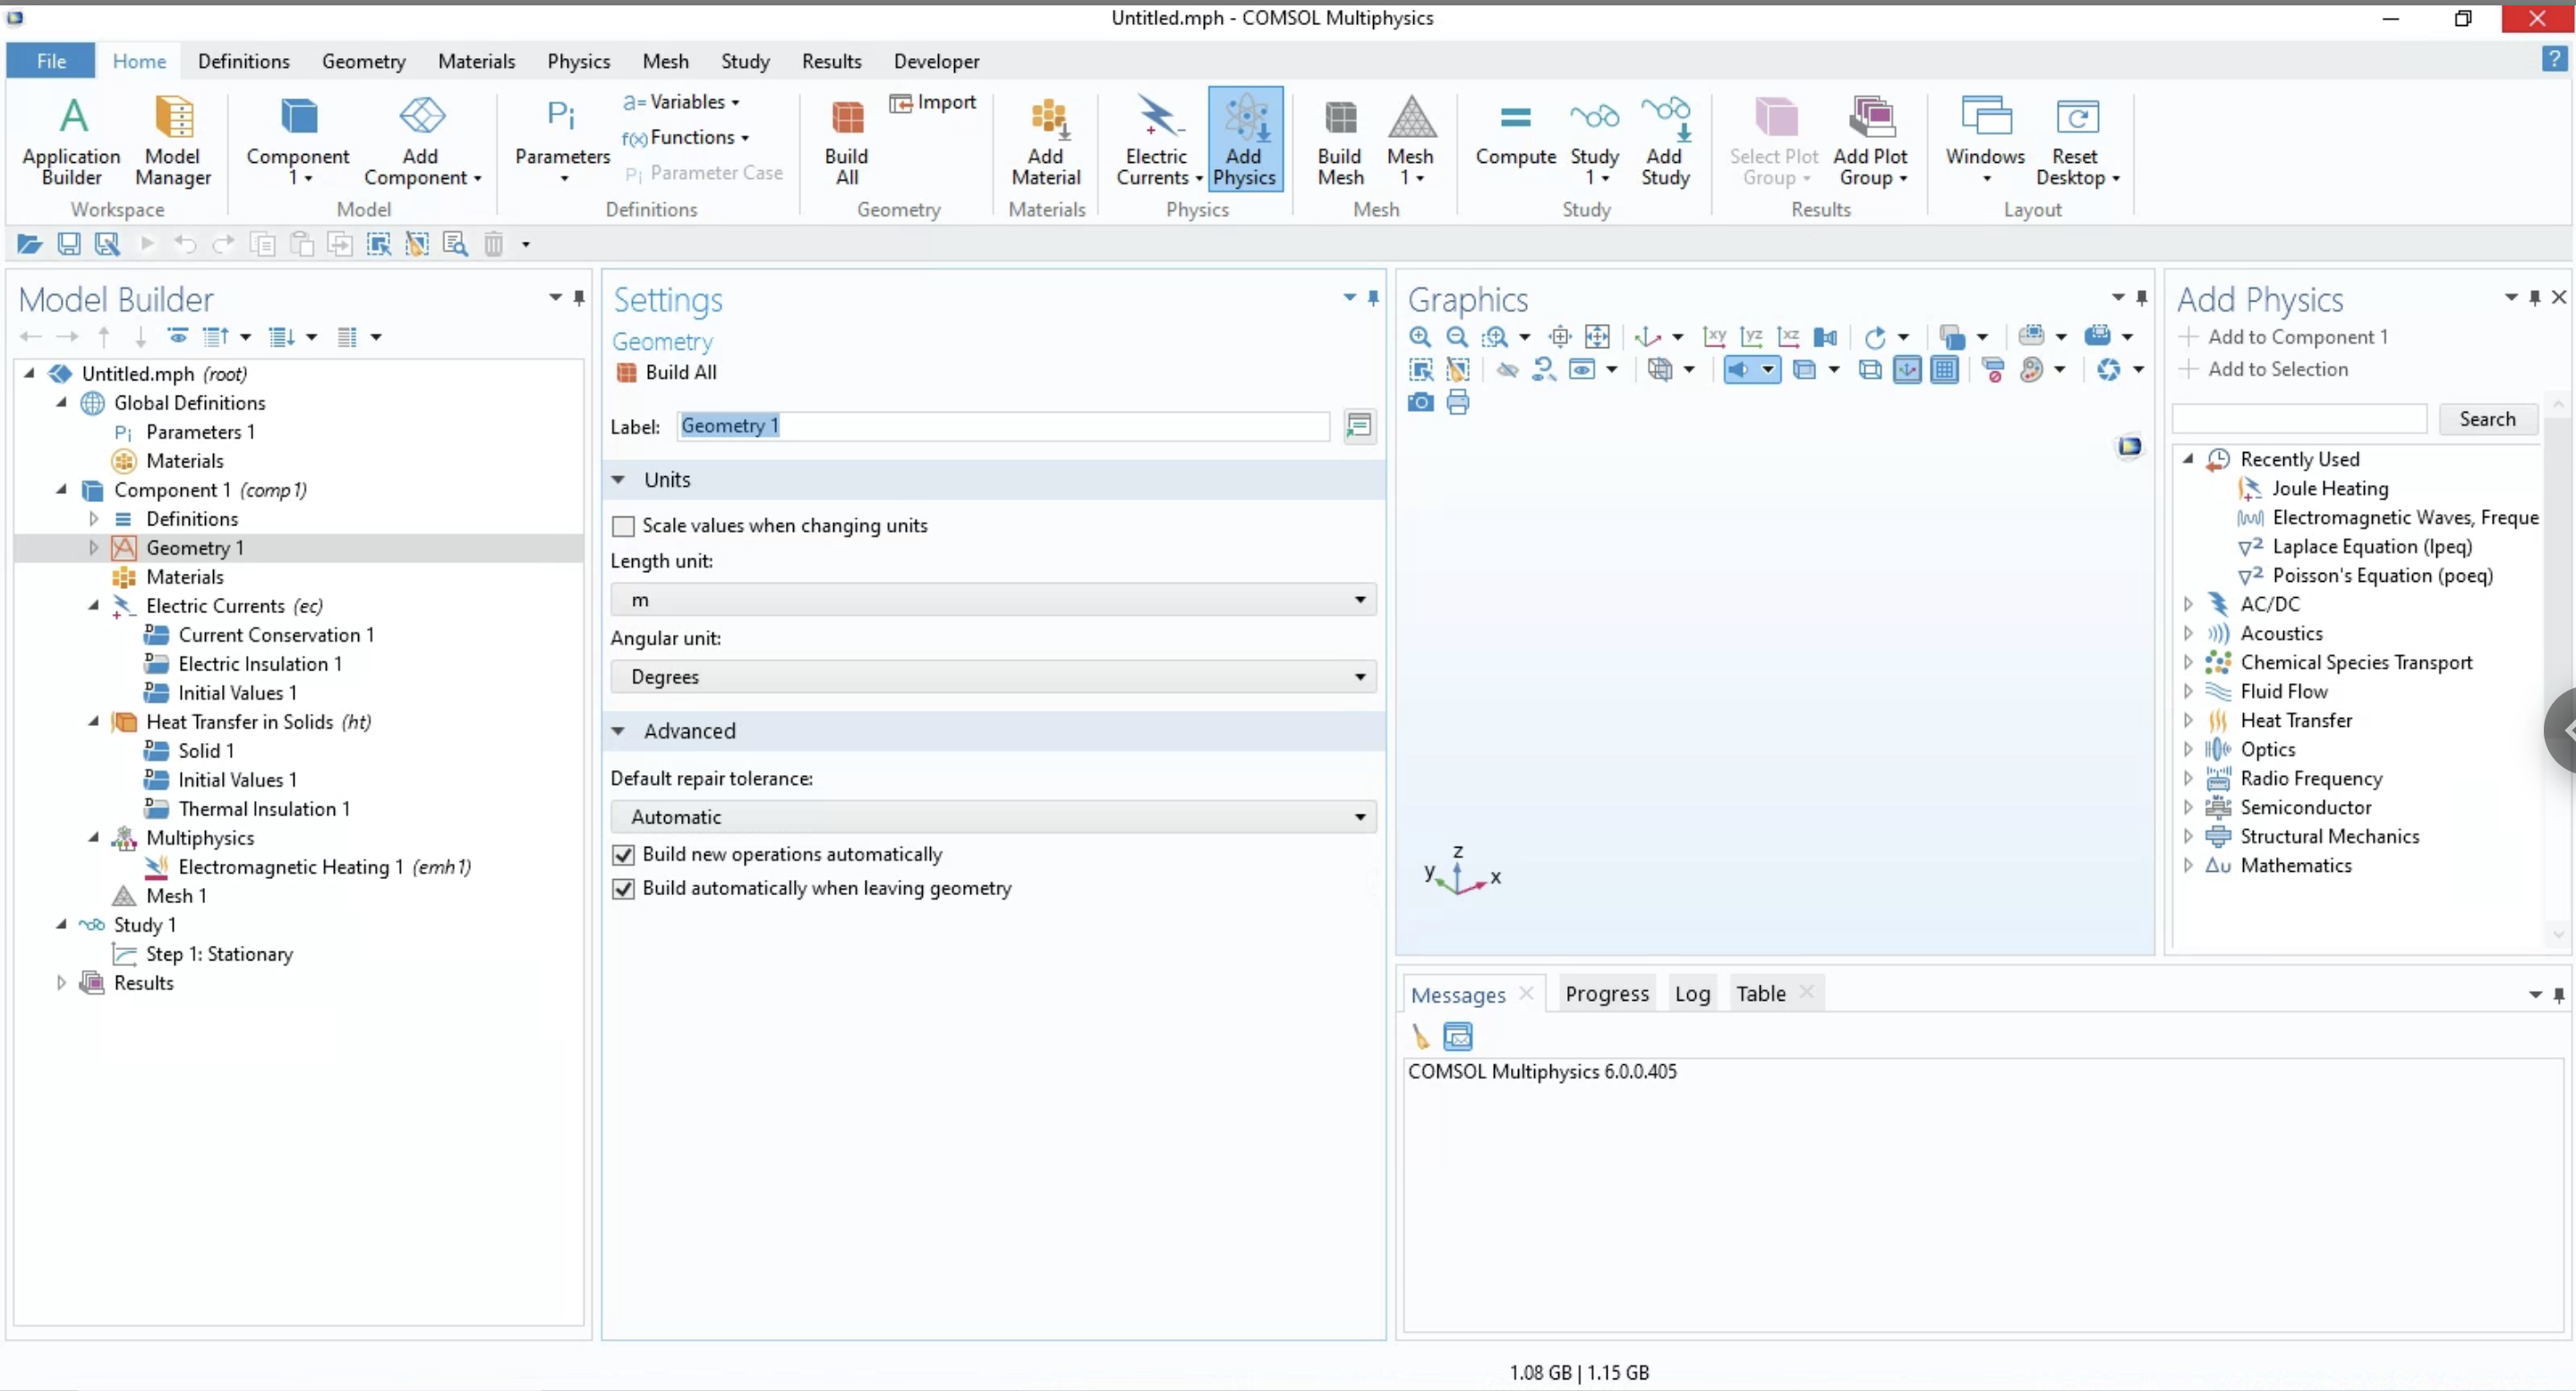
\includegraphics[width=0.4\textwidth]{Chapters/Figures/Chapter 3 Figures/Initial COMSOL Desktop.png}
  \caption{ Source: \cite{}}
  \label{}
\end{figure}

The COMSOL desktop serves as the central hub for constructing and engaging with your model from the ground up. It is designed with an intuitive interface, featuring buttons and ribbons aligned with the modeling process steps. Within the Model Builder window, you'll find the modeling hierarchy, where you have the capability to define your model's dimensions and select specific physics equations for adherence. Additionally, the layout of the COMSOL desktop windows can be customized to suit your preferences.


% SUBSECTION --- Building the Geometry ---
\subsection{Building the Geometry}.
When developing the geometry of your model, multiple pathways are available. You may opt to utilize the drawing tools or geometric shapes provided by COMSOL or import a geometry from an external source.

% TODO: Add "Geometry Button" image
\begin{figure}[ht!]
  \centering
  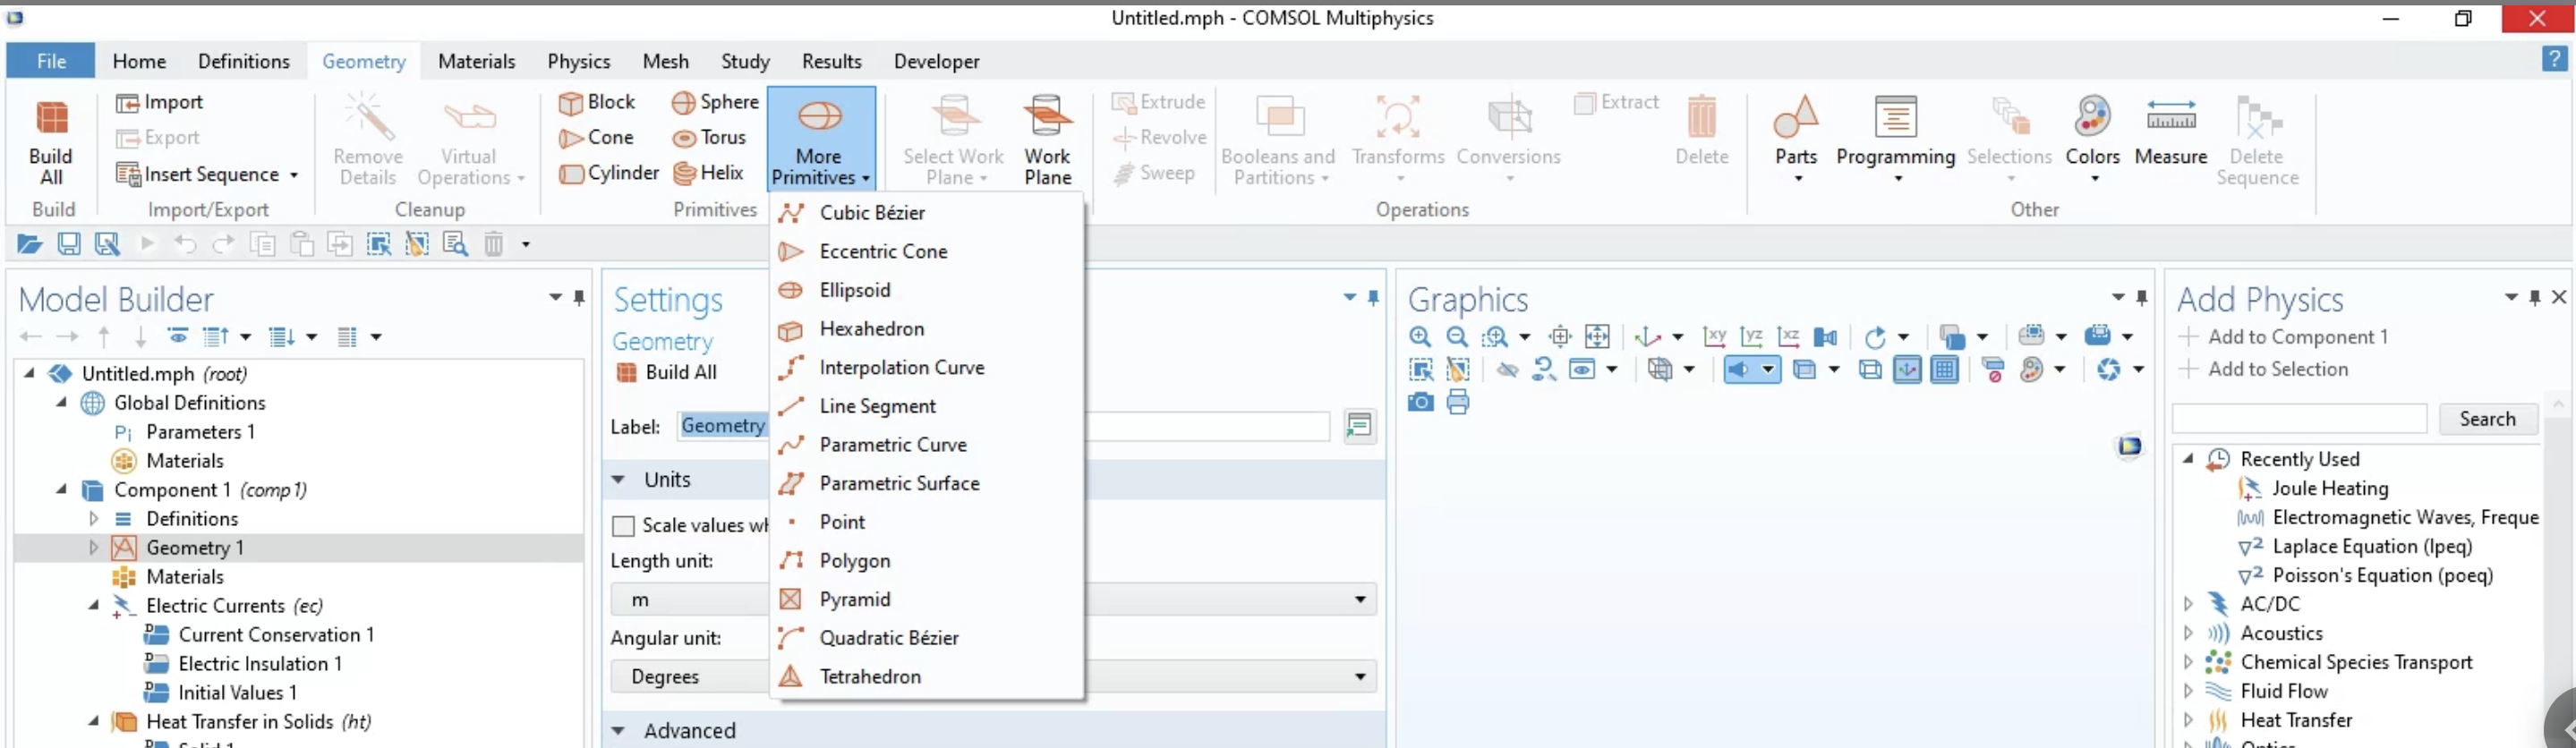
\includegraphics[width=0.4\textwidth]{Chapters/Figures/Chapter 3 Figures/Geometry Tab.png}
  \caption{ Source: \cite{}}
  \label{}
\end{figure}

For this instance, given that the busbar geometry already exists within COMSOL's comprehensive library of pre-configured geometries, accessing this resource simplifies the process. This is achieved by navigating to the File menu and selecting Application Libraries.

% TODO: Add image containing "application libraries" selection
\begin{figure}[ht!]
  \centering
  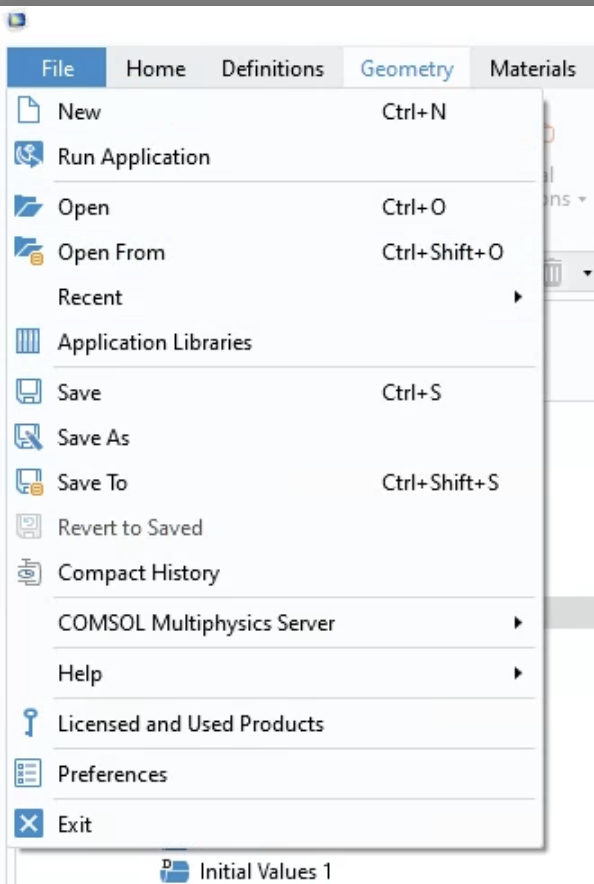
\includegraphics[width=0.4\textwidth]{Chapters/Figures/Chapter 3 Figures/Application Libraries Button.png}
  \caption{ Source: \cite{}}
  \label{}
\end{figure}

Within the Application Libraries, proceed to the COMSOL Multiphysics section, locate the 'busbar\_geom' file, open it, and proceed to save your project accordingly.


% TODO: Add "Application Libraries" image
\begin{figure}[ht!]
  \centering
  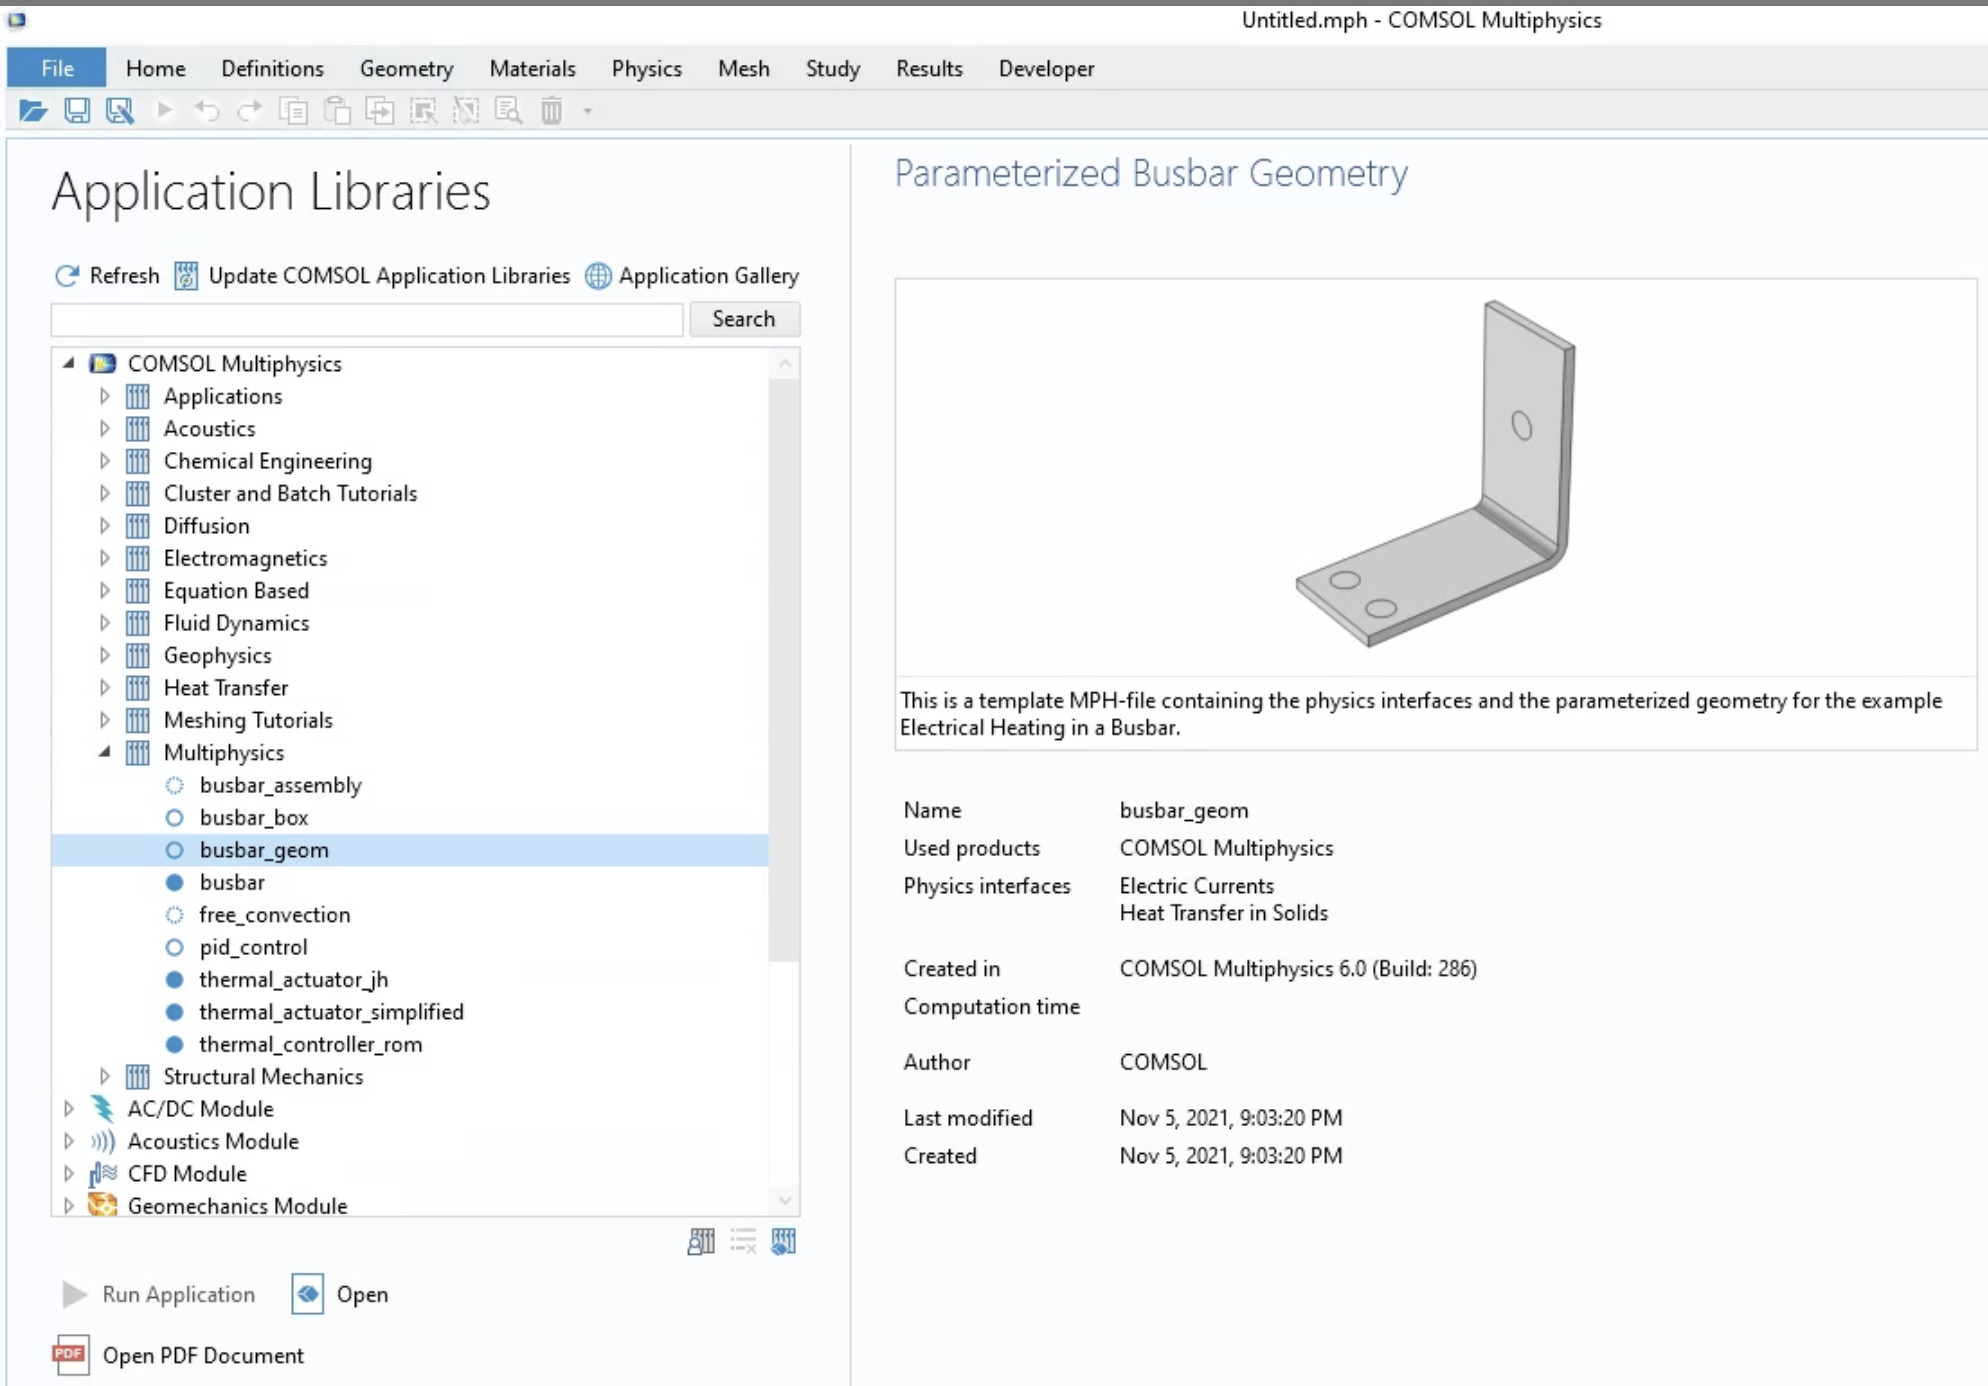
\includegraphics[width=0.4\textwidth]{Chapters/Figures/Chapter 3 Figures/Application Libraries.png}
  \caption{ Source: \cite{}}
  \label{}
\end{figure}

The geometry will now appear in the Graphics window, allowing for zoom and rotational exploration to closely inspect the model. The alteration in the Geometry node within the Model Builder window reflects the sequence of actions executed to construct the busbar geometry. On closer inspection, it becomes evident that specific parameters were employed in crafting this geometry. These parameters are accessible within the "Parameters 1" node, which contains a table detailing the adjustable parameters utilized in the geometry's creation.

% TODO: Add image after when you add default busbar geom to model
\begin{figure}[ht!]
  \centering
  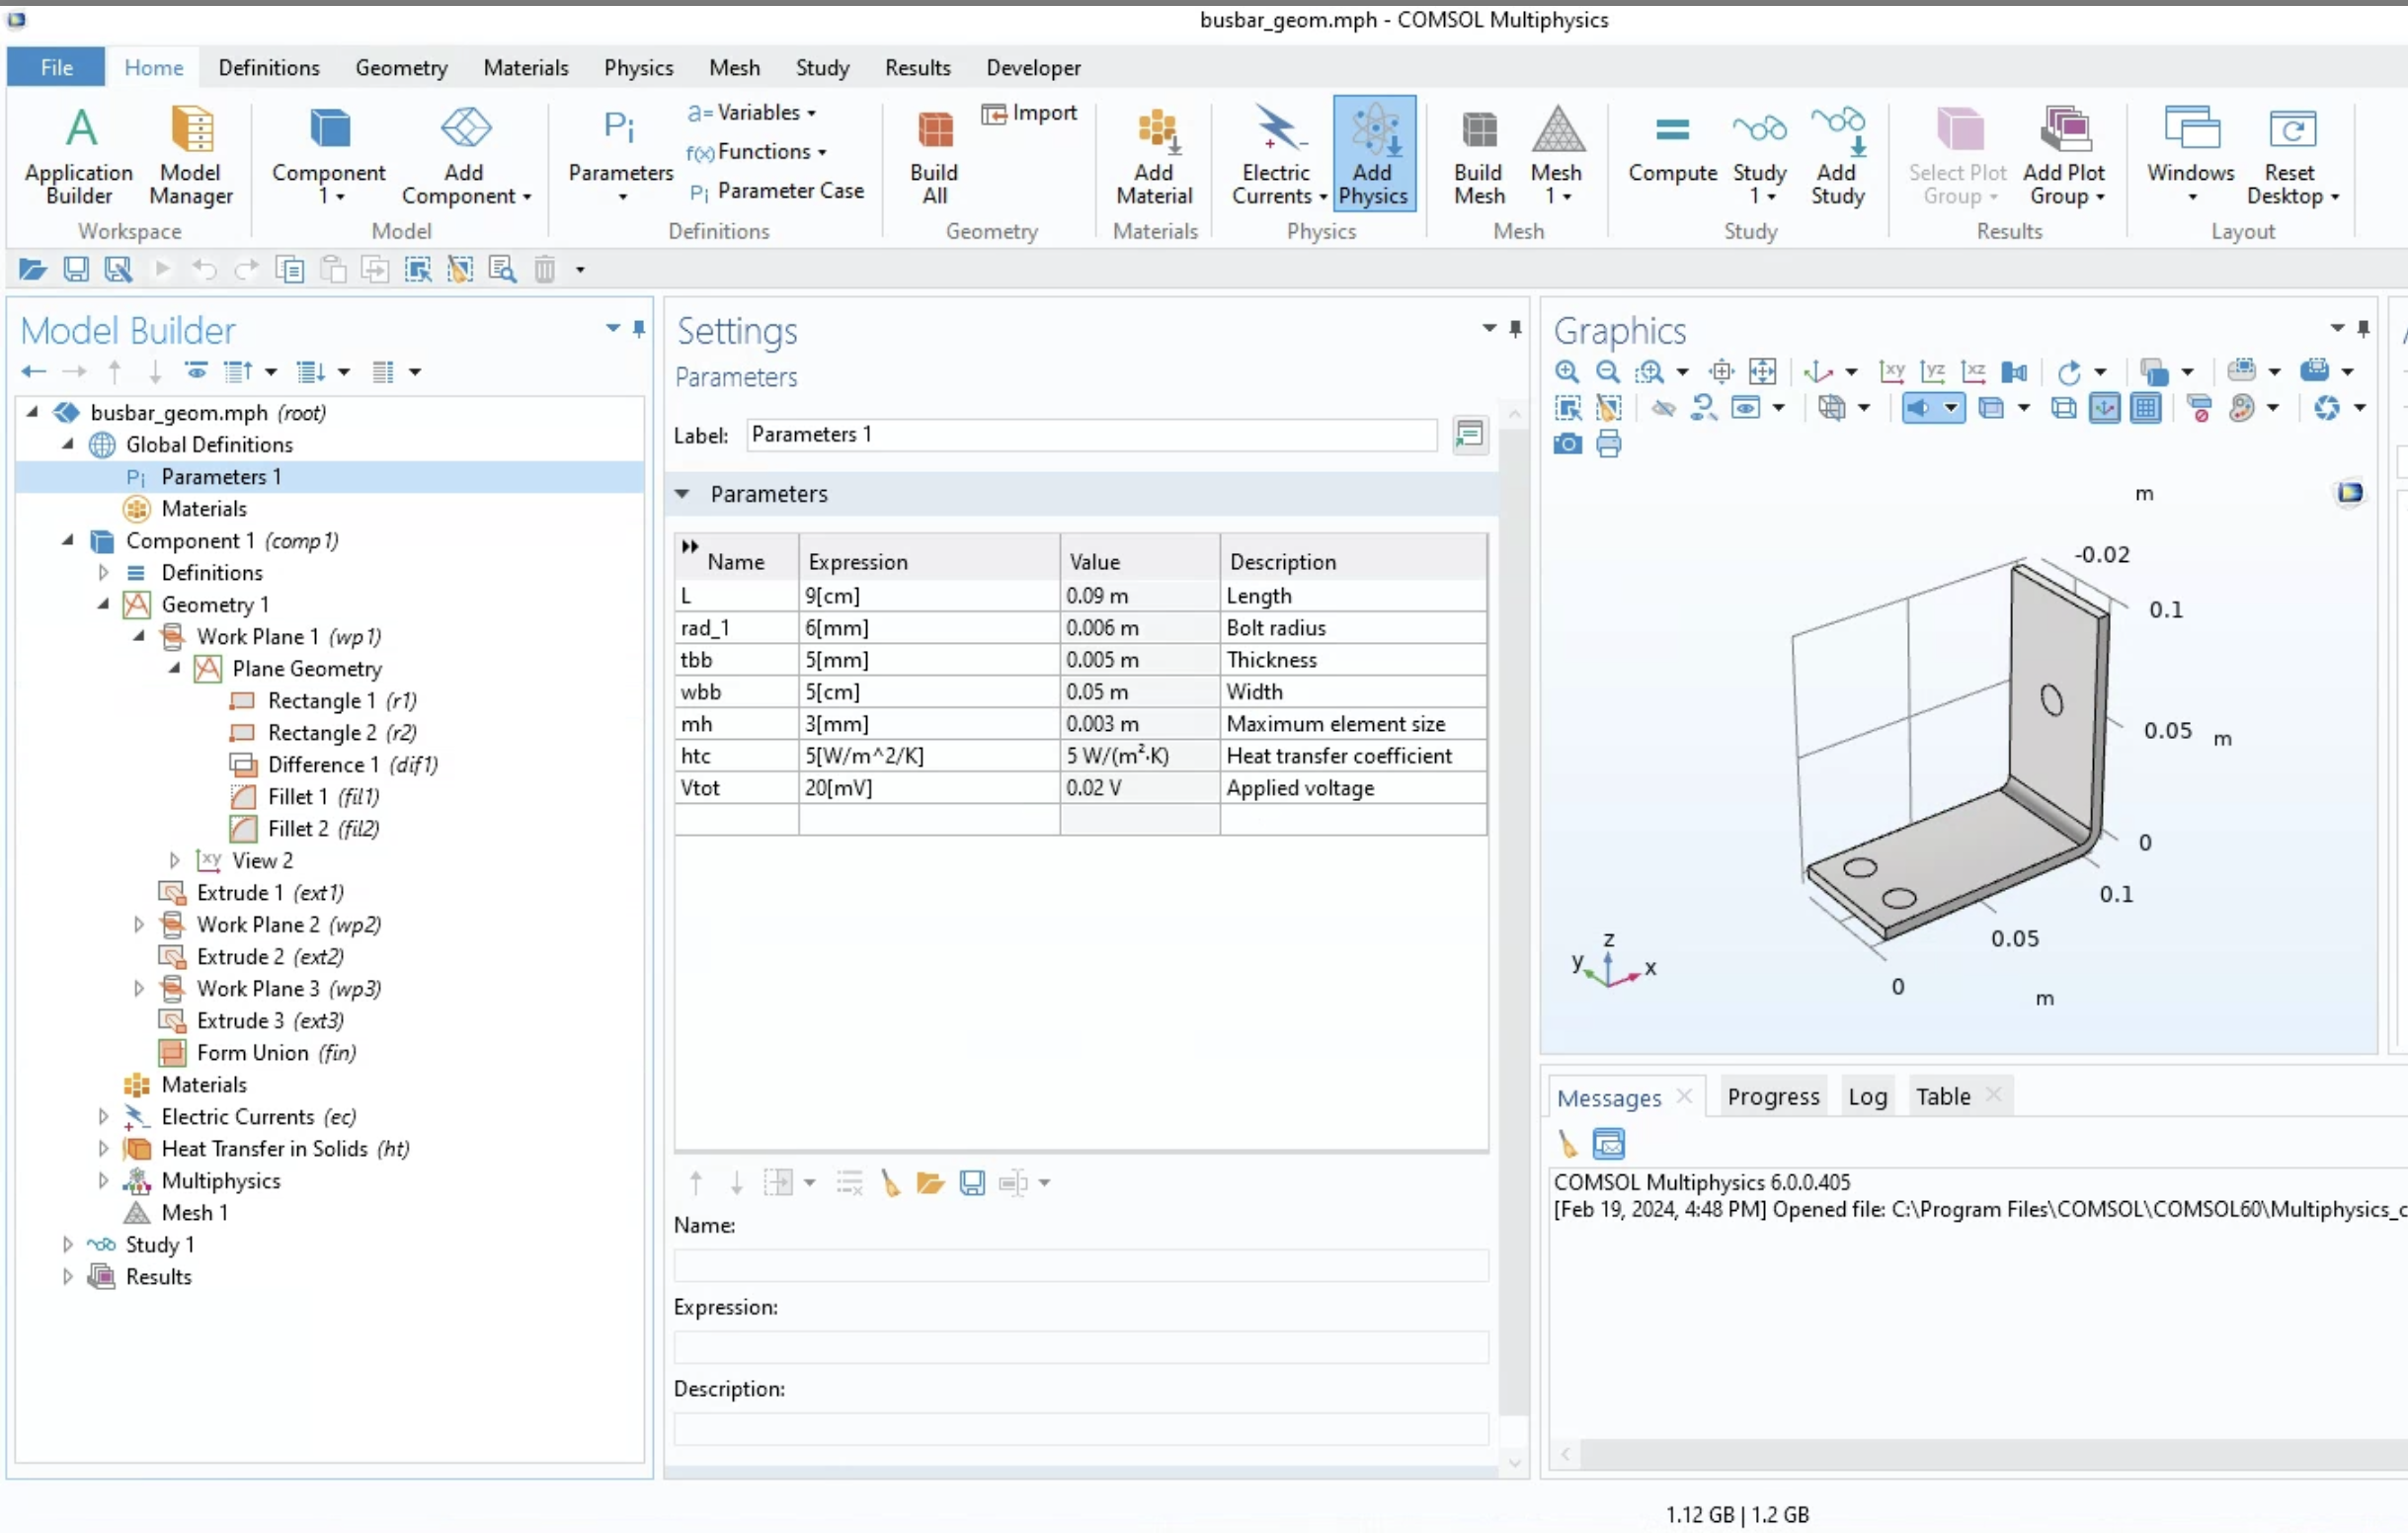
\includegraphics[width=0.4\textwidth]{Chapters/Figures/Chapter 3 Figures/Initial Busbar Geom.png}
  \caption{ Source: \cite{}}
  \label{}
\end{figure}

% SUBSECTION --- Specifying the Material Properties ---
\subsection{Specifying the Material Properties}.

Our busbar comprises various components each requiring distinct materials, necessitating batch assignment of materials to selected parts rather than individual allocation. To commence, access the Definitions tab and opt for the Explicit selection.

% TODO: Add explicit choice selection from Definitions tab
\begin{figure}[ht!]
  \centering
  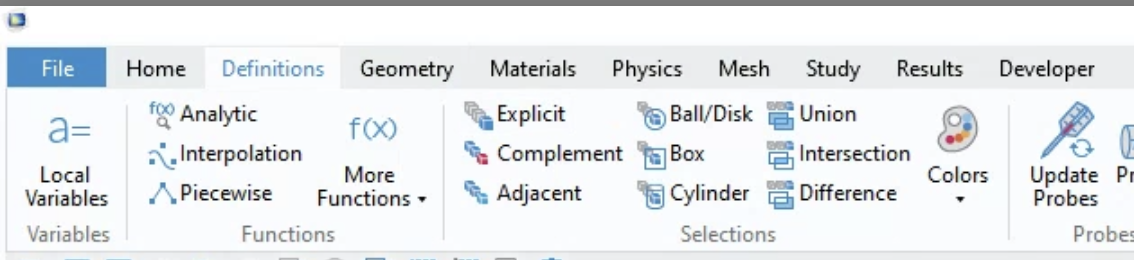
\includegraphics[width=0.4\textwidth]{Chapters/Figures/Chapter 3 Figures/Explicit Choice Selection from Definitions Tab.png}
  \caption{ Source: \cite{}}
  \label{}
\end{figure}

Following this, in the Graphics window, we identify and select the bolts, ensuring both their front and back sides are chosen due to their differing material composition from the busbar's main body.

% TODO: Add bolt selections after selections
\begin{figure}[ht!]
  \centering
  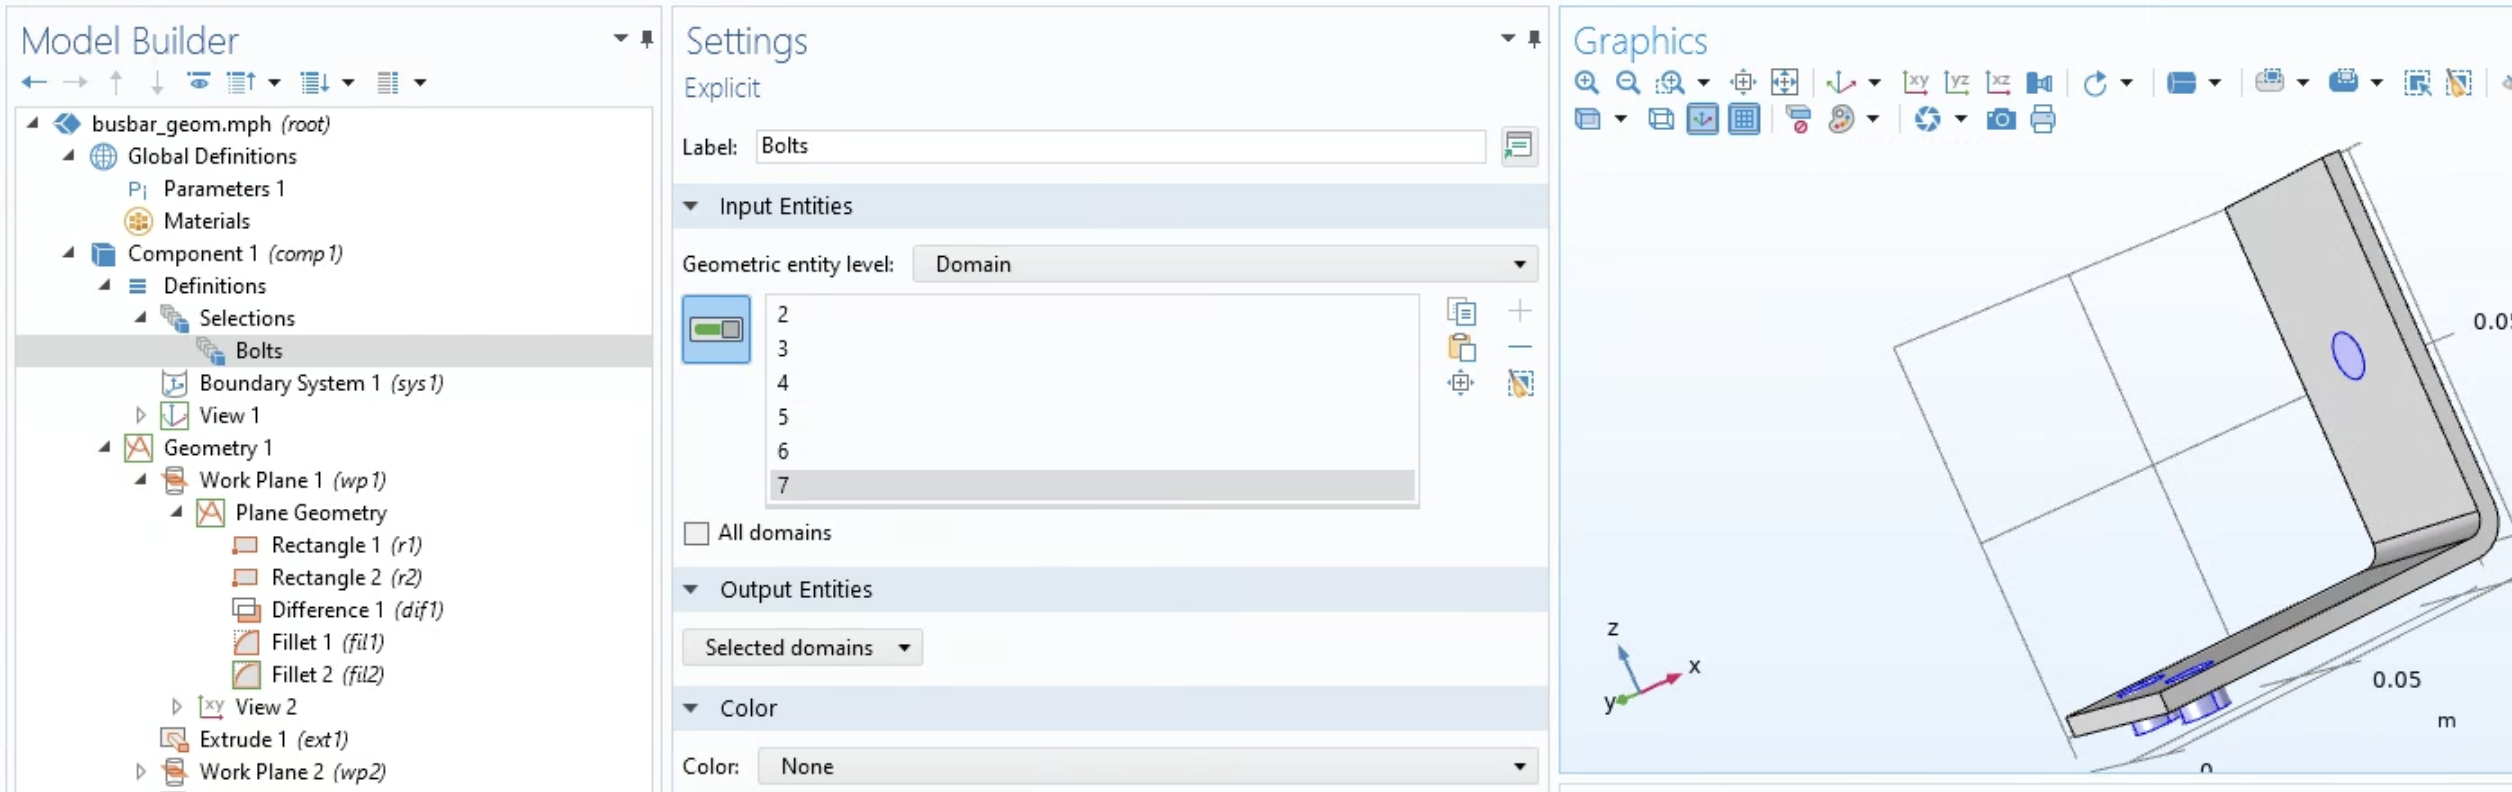
\includegraphics[width=0.4\textwidth]{Chapters/Figures/Chapter 3 Figures/Bolts Selection.png}
  \caption{ Source: \cite{}}
  \label{}
\end{figure}

Proceeding to material assignment, we move to the Materials ribbon and select the Add Materials feature. This action opens the "Add Material" window, offering a selection of materials to apply to the chosen components.

%-----------------HERE------------

% TODO: Add the Add Materials image
\begin{figure}[ht!]
  \centering
  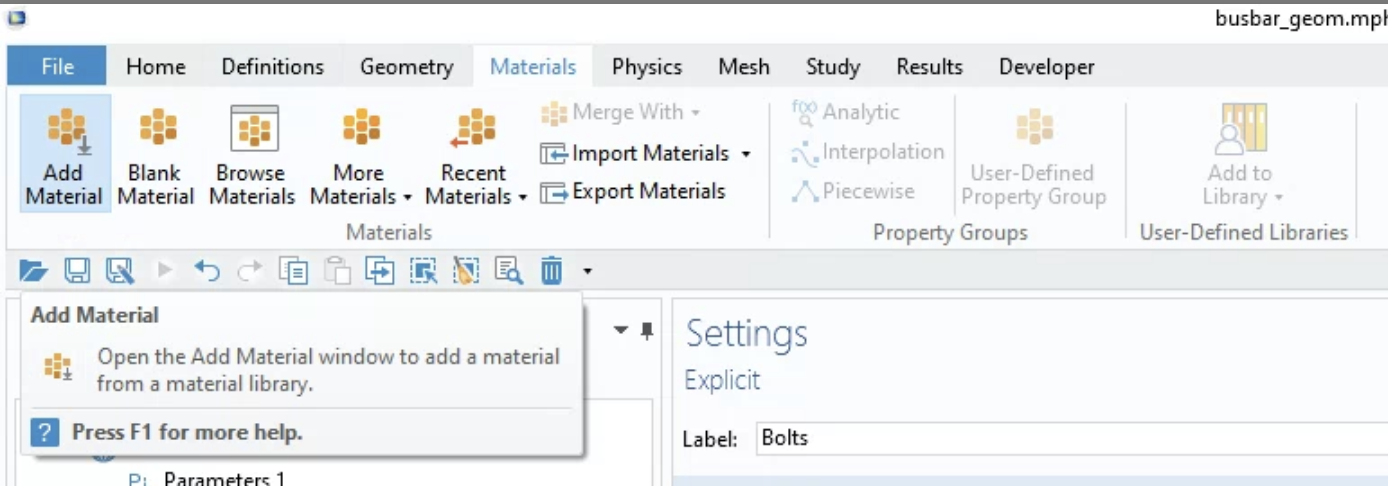
\includegraphics[width=0.4\textwidth]{Chapters/Figures/Chapter 3 Figures/Add Material Button.png}
  \caption{Source: \cite{}}
  \label{}
\end{figure}

Choose the Built-In node and select the Titanium (for the bolts) and Copper materials.

% TODO: Add the Add Materials window image
\begin{figure}[ht!]
  \centering
  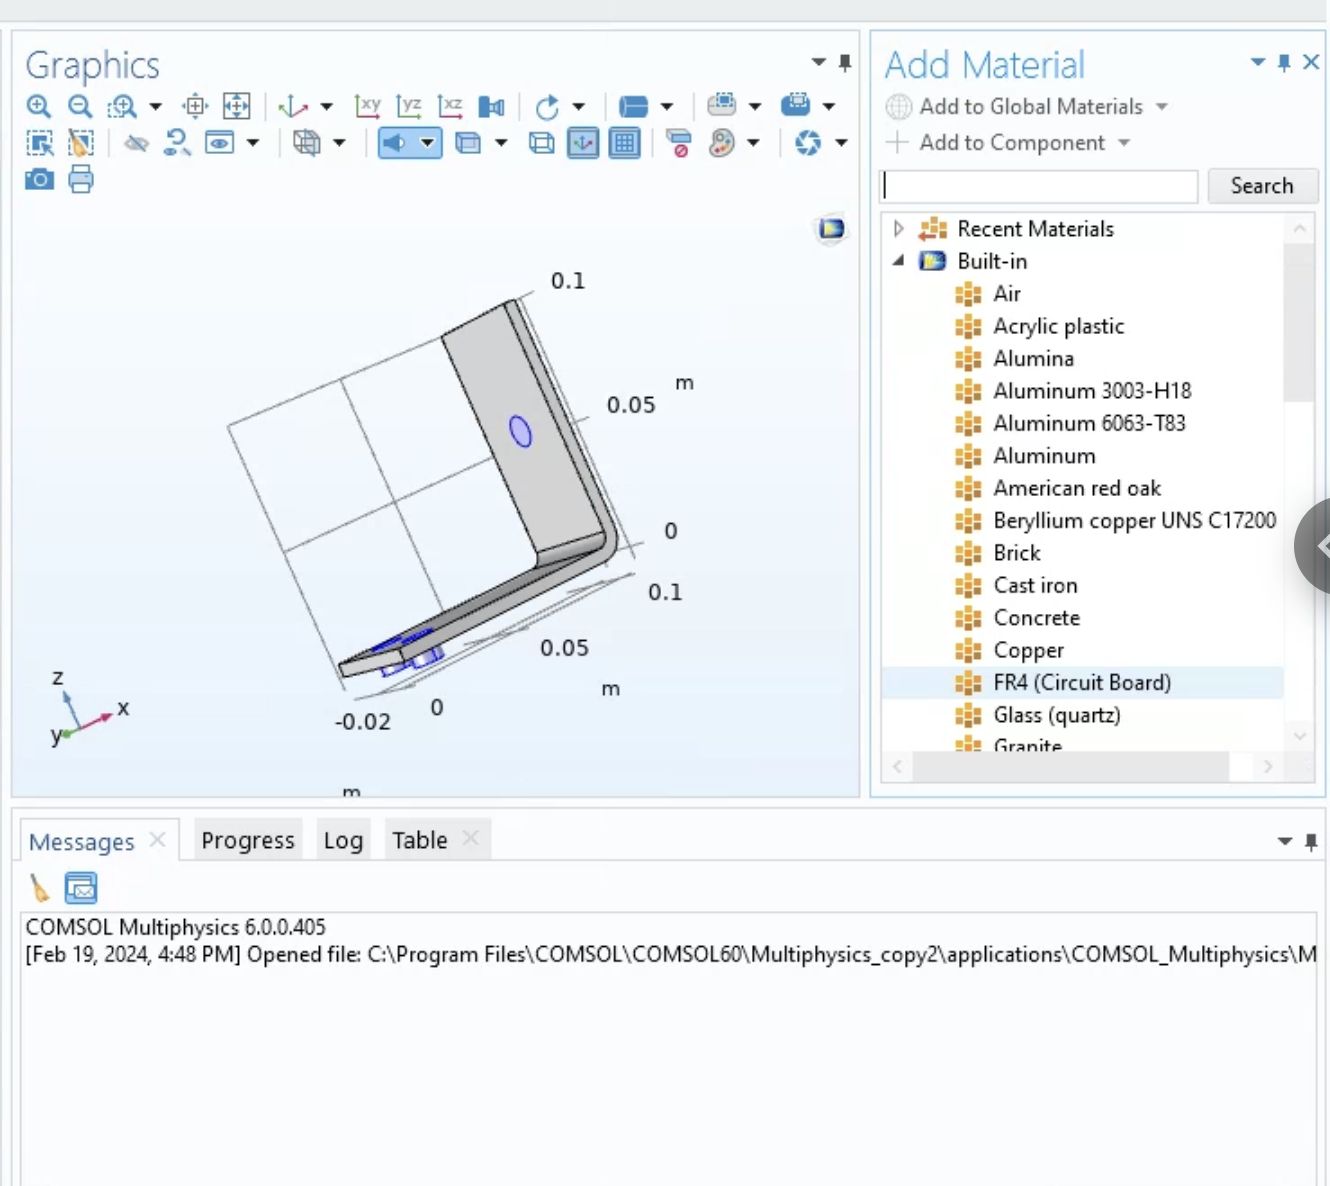
\includegraphics[width=0.4\textwidth]{Chapters/Figures/Chapter 3 Figures/Add Material Window.png}
  \caption{Source: \cite{}}
  \label{}
\end{figure}

The Bolts selections definition we made earlier comes in handy when we assign every bolt to the Titanium material by choosing the Bolts selection as shown below

% TODO: Add the bolts for titanium material selection
\begin{figure}[ht!]
  \centering
  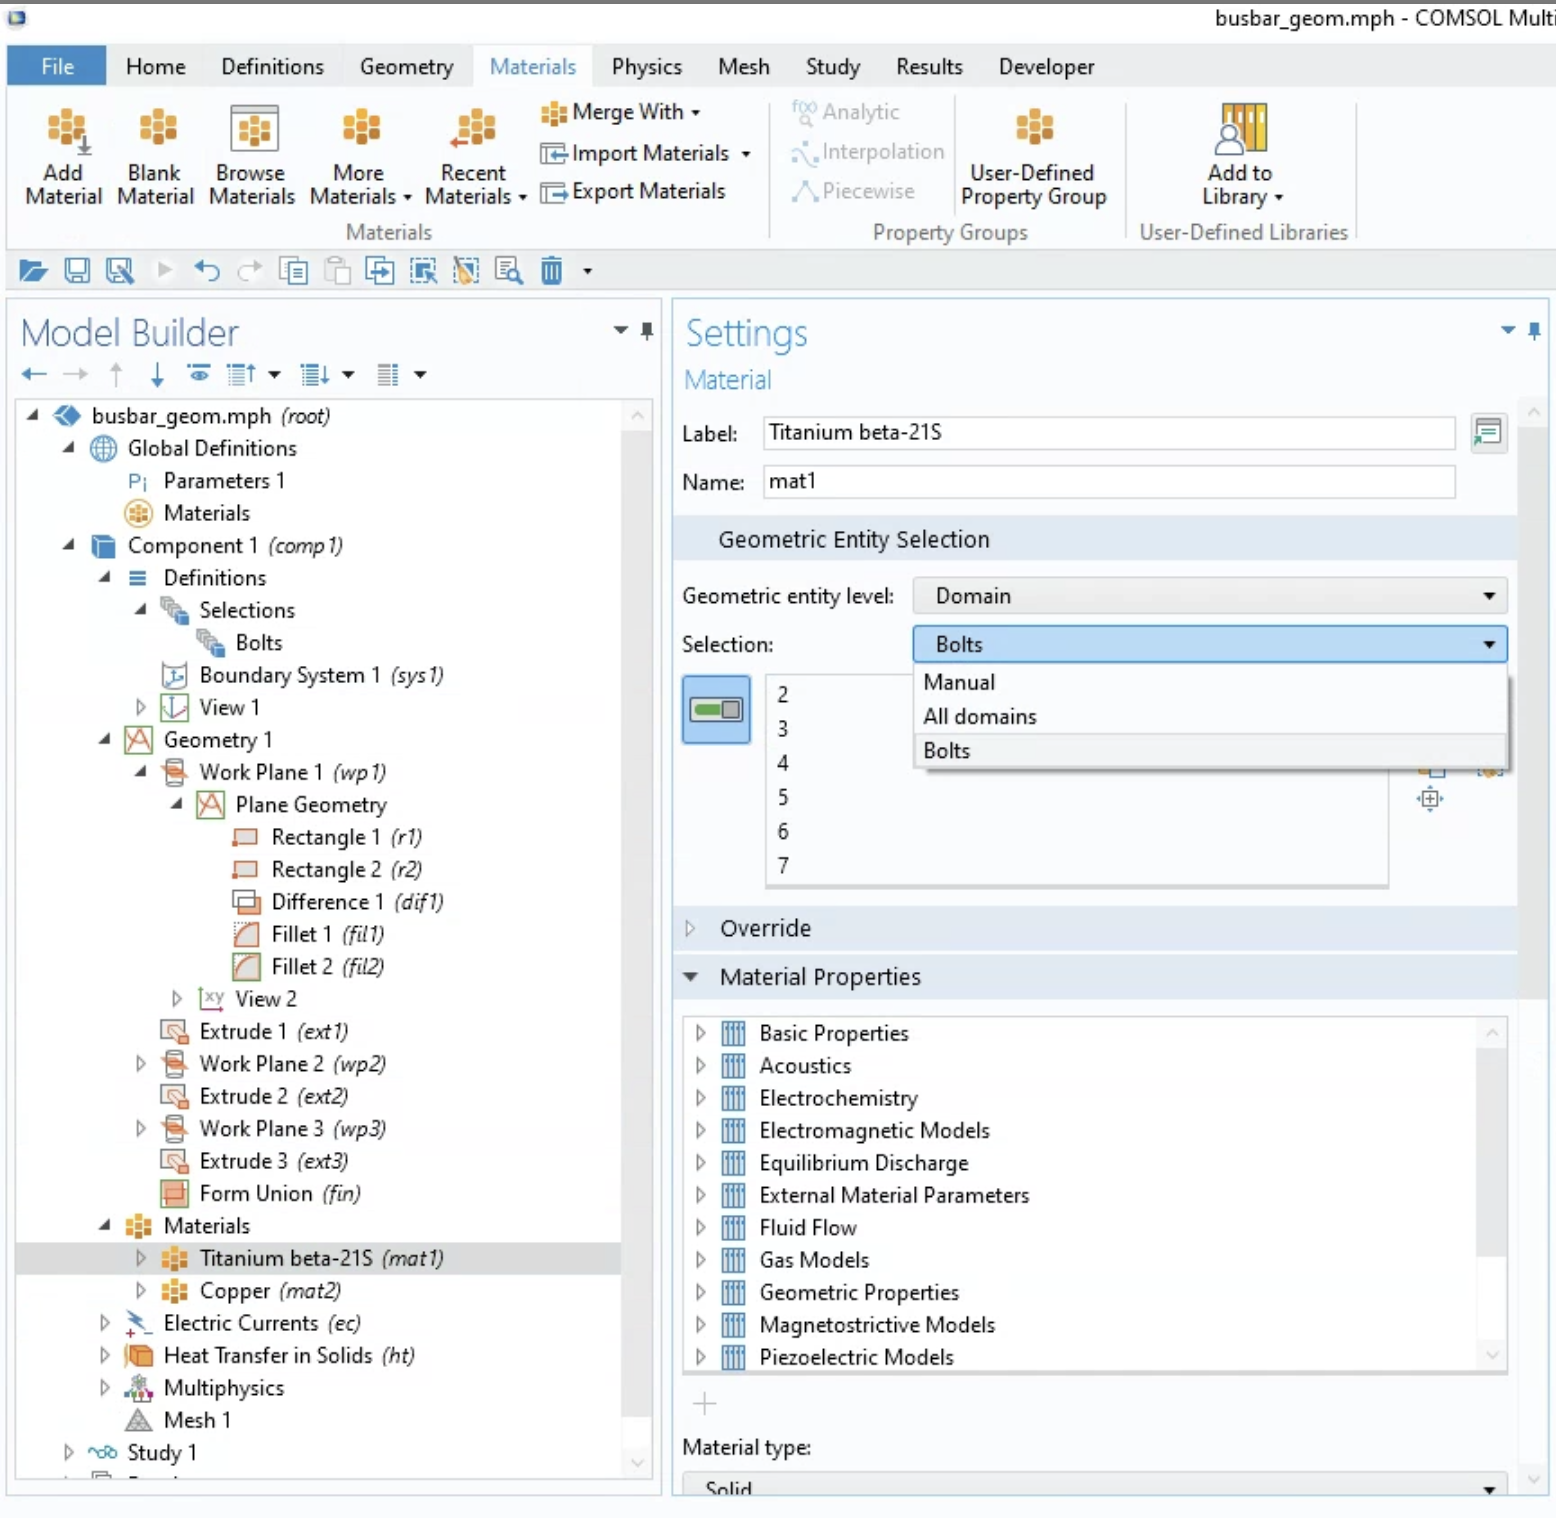
\includegraphics[width=0.4\textwidth]{Chapters/Figures/Chapter 3 Figures/Bolts Selection Choice.png}
  \caption{Source: \cite{}}
  \label{}
\end{figure}

With each material addition, and thus, material node addition in the Model Builder window comes a table in the Settings window of the Material Contents which contain the physical properties of said materials, such as, Electrical Conductivity, Heat Capacity, among others.

% TODO: Add image showing material contents (properties)
\begin{figure}[ht!]
  \centering
  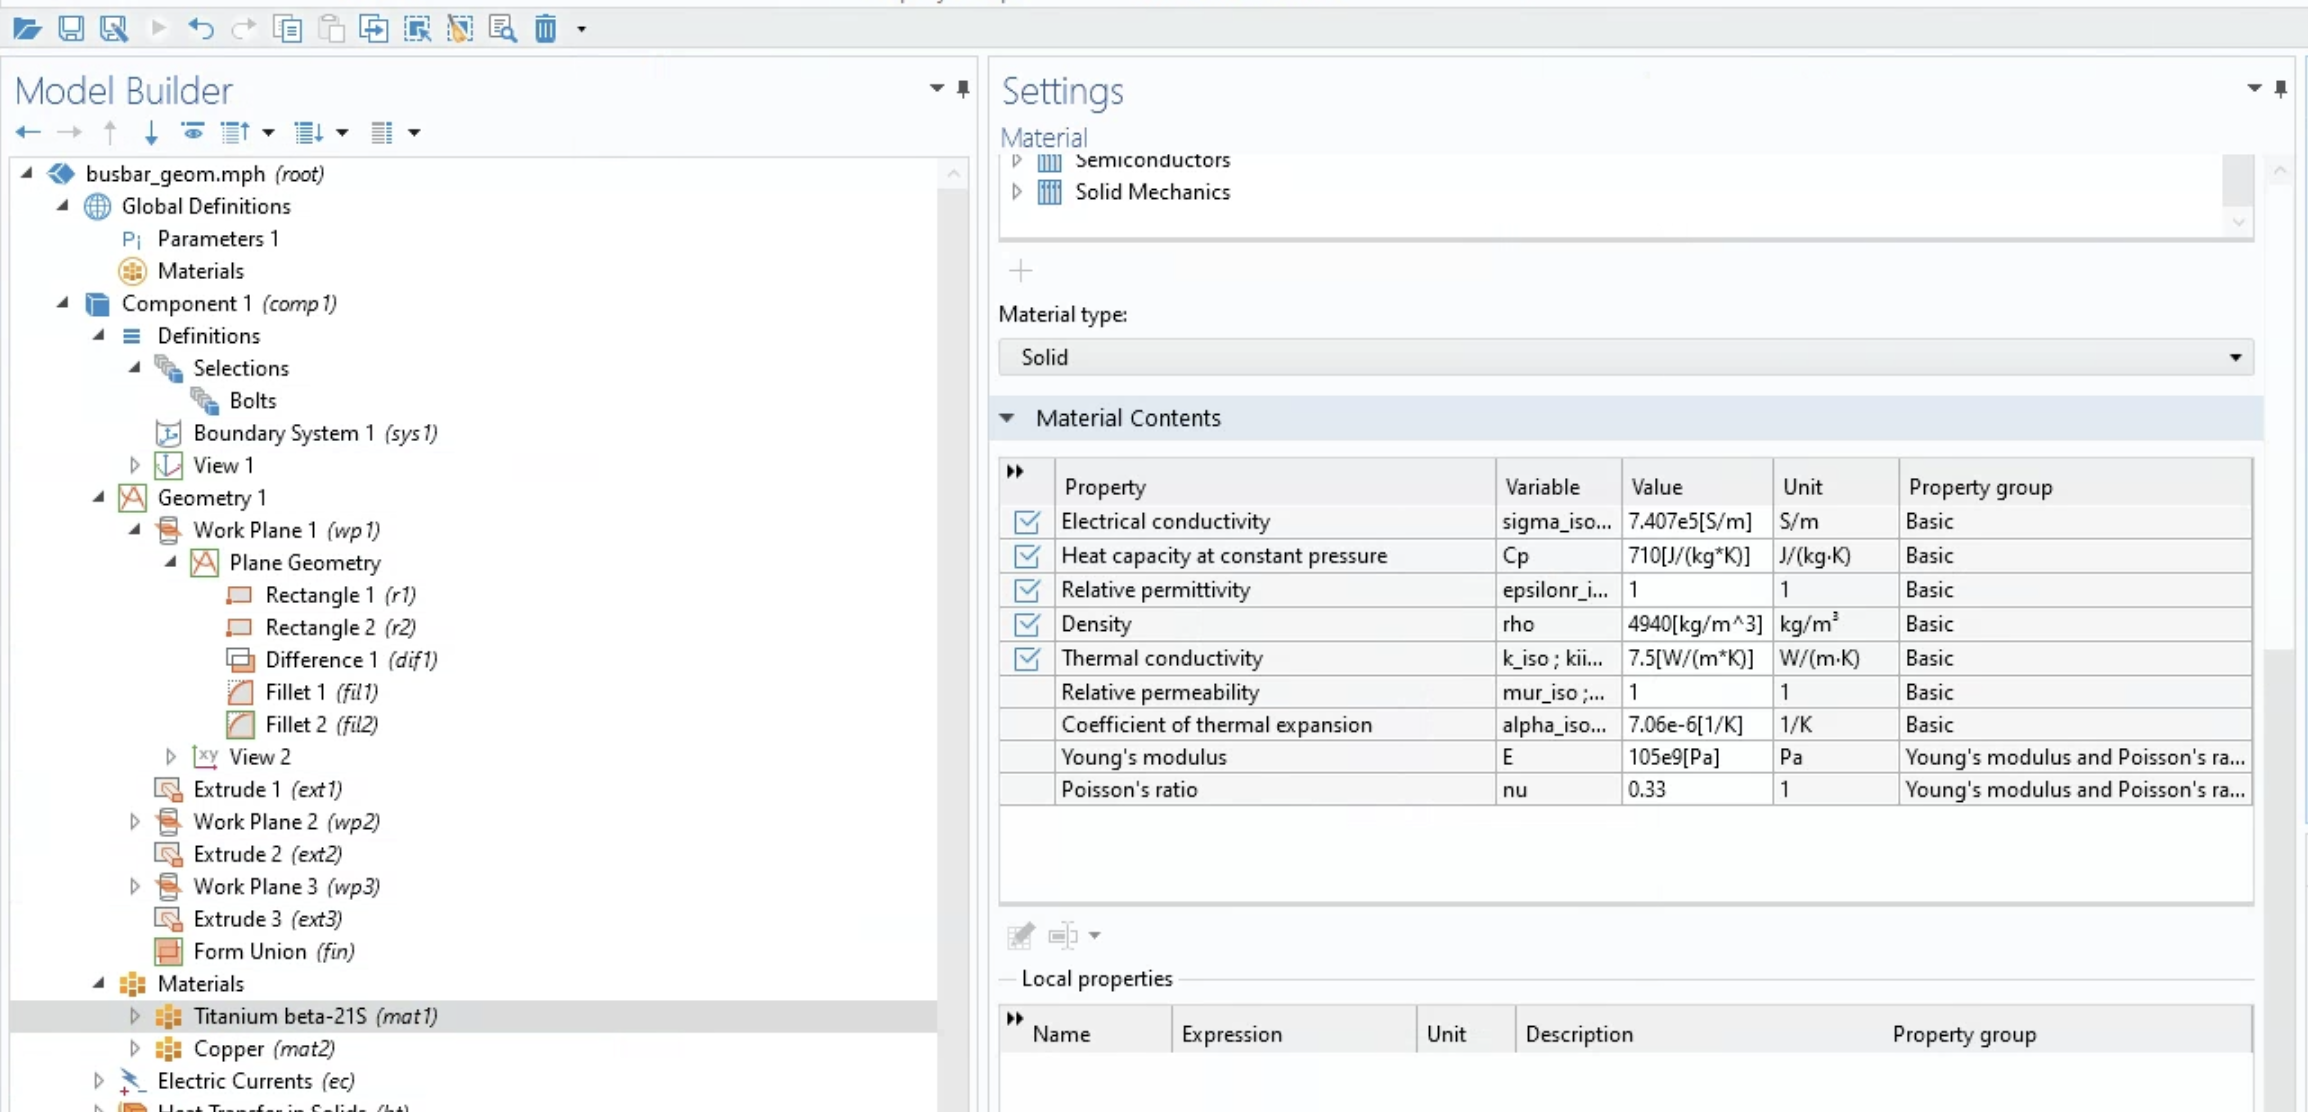
\includegraphics[width=0.4\textwidth]{Chapters/Figures/Chapter 3 Figures/Material Contents in Settings Window.png}
  \caption{Source: \cite{}}
  \label{}
\end{figure}


% SUBSECTION --- Defining the Physics Boundary Conditions ---
\subsection{Defining the Physics Boundary Conditions}.
We can now start assigning mathematical equations to different parts of our geometry or model in order to simulate our Physics and we do this by selecting parts of the geometry and then specifying appropriate equations and physical conditions that describe that part.

Let's start by configuring the Physics for the electric currents interface which will simulate the conduction of electric current from the single bolt to the pair of bolts on the other end of the busbar. Depending on the Physics you selected when setting up the model environment, some equations may be built-in to your Physics nodes, for instance, if you navigate to the "Electric Currents (ec)" node, you can see the corresponding equations detailed in the Settings window. One of the equations is the ubiquitous equation relating the electric field to the electric potential, $\mathbf{E} = -\nabla V$.

% TODO: Add image showing equation
\begin{figure}[ht!]
  \centering
  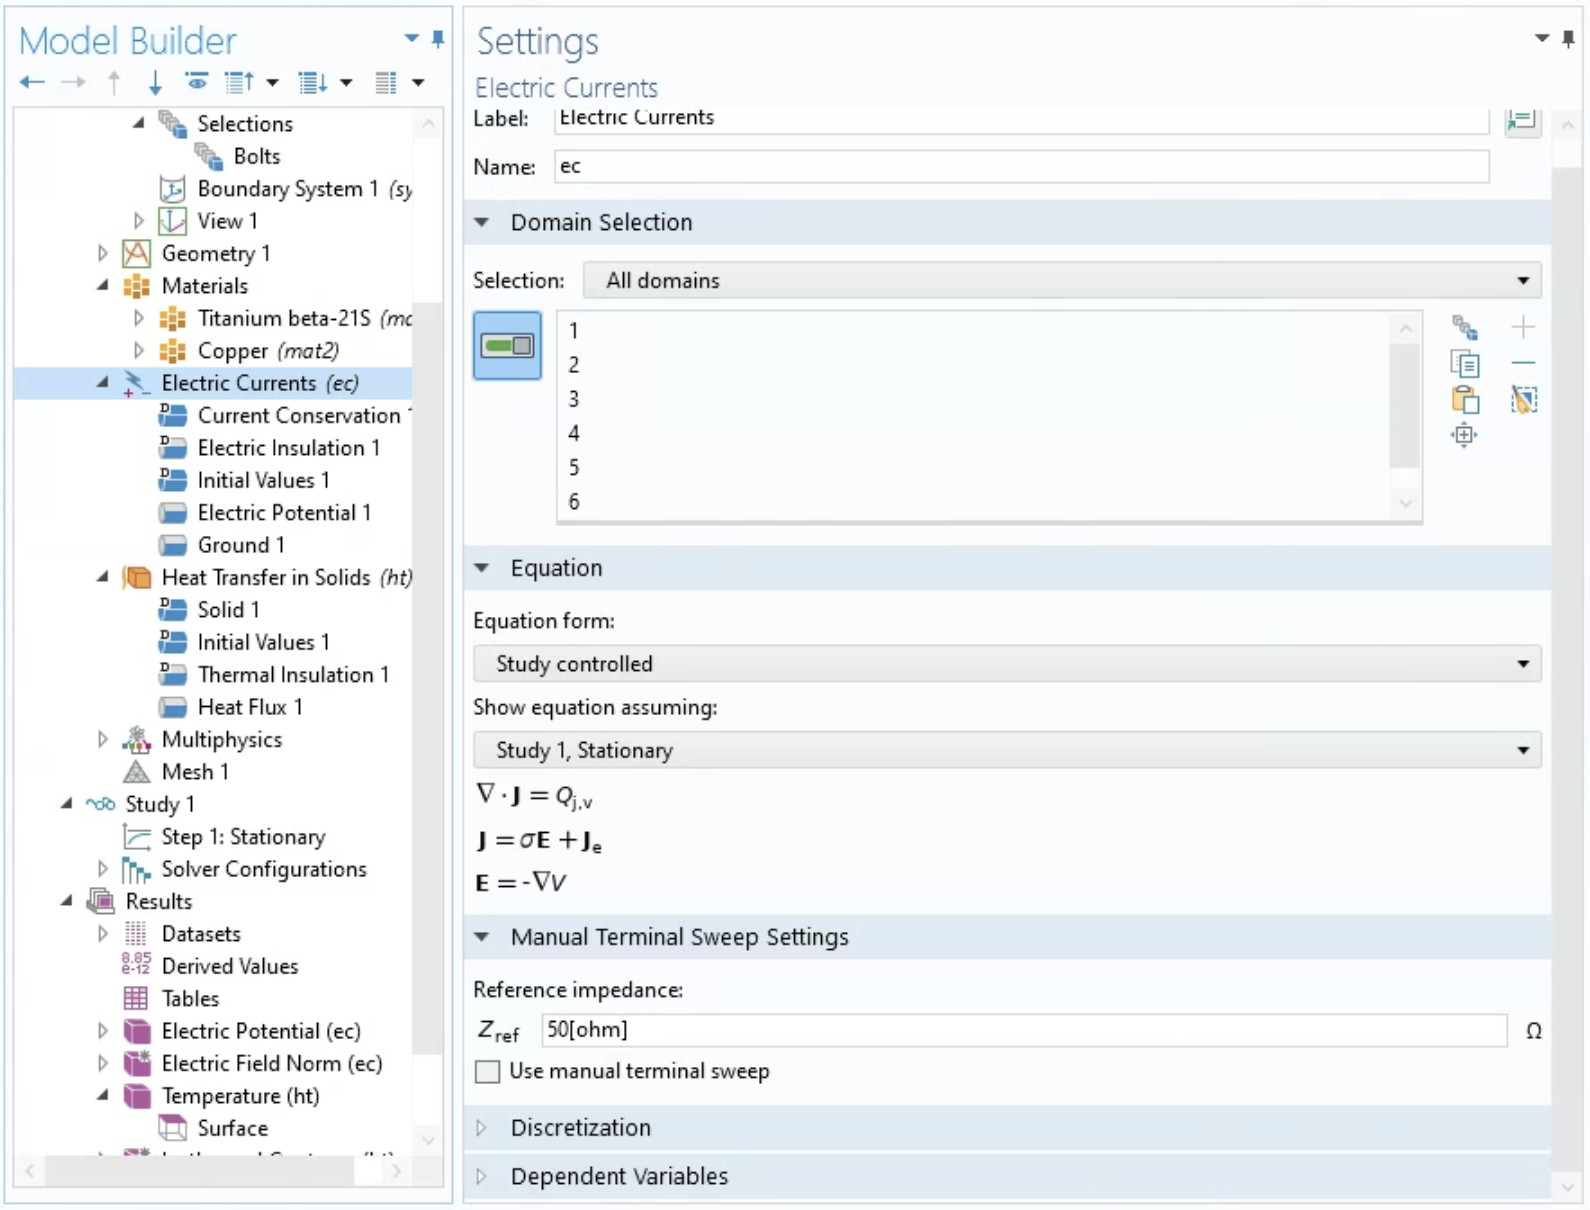
\includegraphics[width=0.4\textwidth]{Chapters/Figures/Chapter 3 Figures/Electrical Currents Physics Equation.png}
  \caption{Source: \cite{}}
  \label{}
\end{figure}

So there's no black box in COMSOL Multiphysics since the user can always know what COMSOL Multiphysics is doing and how.

When we added the physics to our model, this also included a few default nodes under each respective physics nodes and we only add the boundary conditions and constraints to our model when they are different from these default nodes. So for instance, for the "Electric Currents (ec)" Physics, you have default boundary conditions such as "Electric Insulation 1" which is default and applied to all boundaries. This is not valid for the case of our model.

We want to apply a voltage to the the bottom surface of the single bolt. To do this, we click on the Physics tab, click Boundaries, and select Electric Potential and upon selecting it, you'll see an Electric Potential 1 node was added. We now need to select the select the piece of geometry this potential applies to, and as stated before, we hover over the surface we want to select and click it. For the value of electric potential, we want to apply a voltage of 20 mV, to which you enter as 20[mV] where the brackets specify the units if different from the default.

To make your life easier though, recall that in the Parameters table in the "Parameters 1" node, we have a variable Vtot, that included the value for the applied voltage so instead of manually writing 20[mV], you could just type the variable name. Doing this will allow you to set up a parametric study later on.

Lastly, we want to include a ground boundary condition to the bottom surface of each pair of bolts on the other side of the busbar. To do this, we can click the boundaries button in the Physics tab and select Ground and select the appropriate parts of the geometry.

% TODO: Add image showing "Electric Currents" boundary conditions
\begin{figure}[ht!]
  \centering
  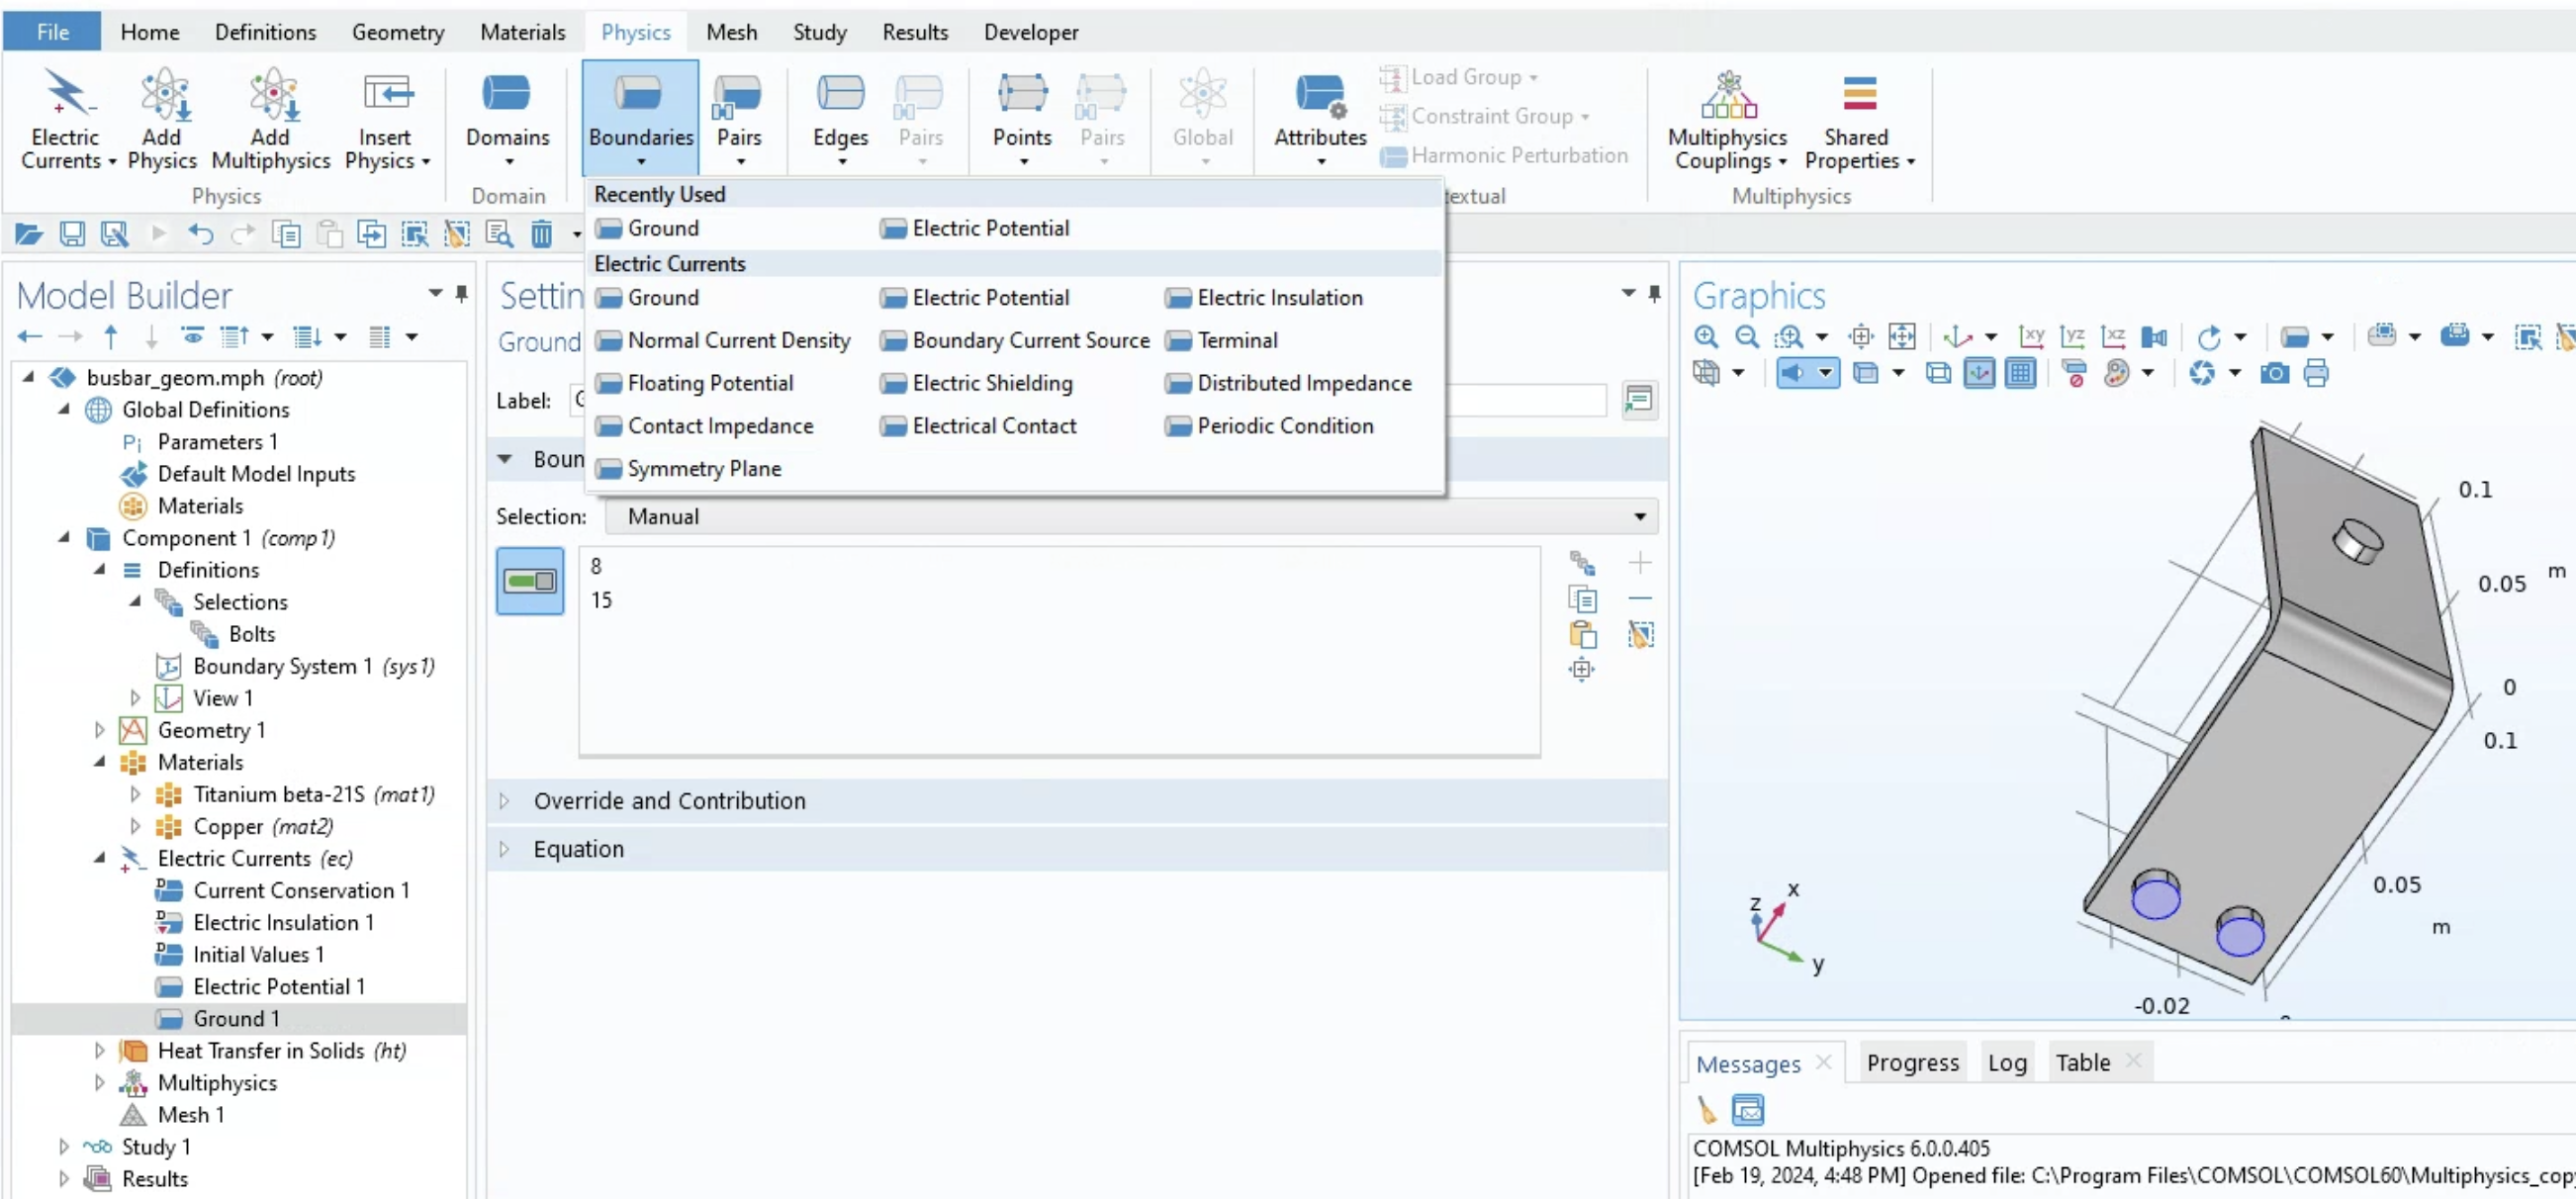
\includegraphics[width=0.4\textwidth]{Chapters/Figures/Chapter 3 Figures/Electric Currents Boundary Conditions.png}
  \caption{Source: \cite{}}
  \label{}
\end{figure}

Since the Joule Heating physics option we selected was a coupled one, we also need to specify the boundary conditions for the thermal portion of our model. Again, here the "Thermal Insulation 1" boundary condition is applied to all part of our model which is not valid in our case. Navigate to the Physics tab then Boundaries, and then select Heat Flux. In the settings window, in the Boundary Selection option, select, "All Boundaries" and omit all the bolt surfaces we selected earlier for the Electric Currents boundary conditions, that is, boundaries 8, 15, and 43. You can do this by selecting these boundary numbers and clicking on the minus sign which is "Remove from Selection".

Under the Heat Flux section, we're going to select the "Convective heat flux" option under "Flux Type" and we want to enter a value of 5 $W/(m^2\cdot K)$. But like we did for the electric potential, we just refer back to the Parameters 1 node, and type in htc which specifies the value of 5 $W/(m^2\cdot K)$.

% TODO: Add image showing Heat Flux boundary conditions
\begin{figure}[ht!]
  \centering
  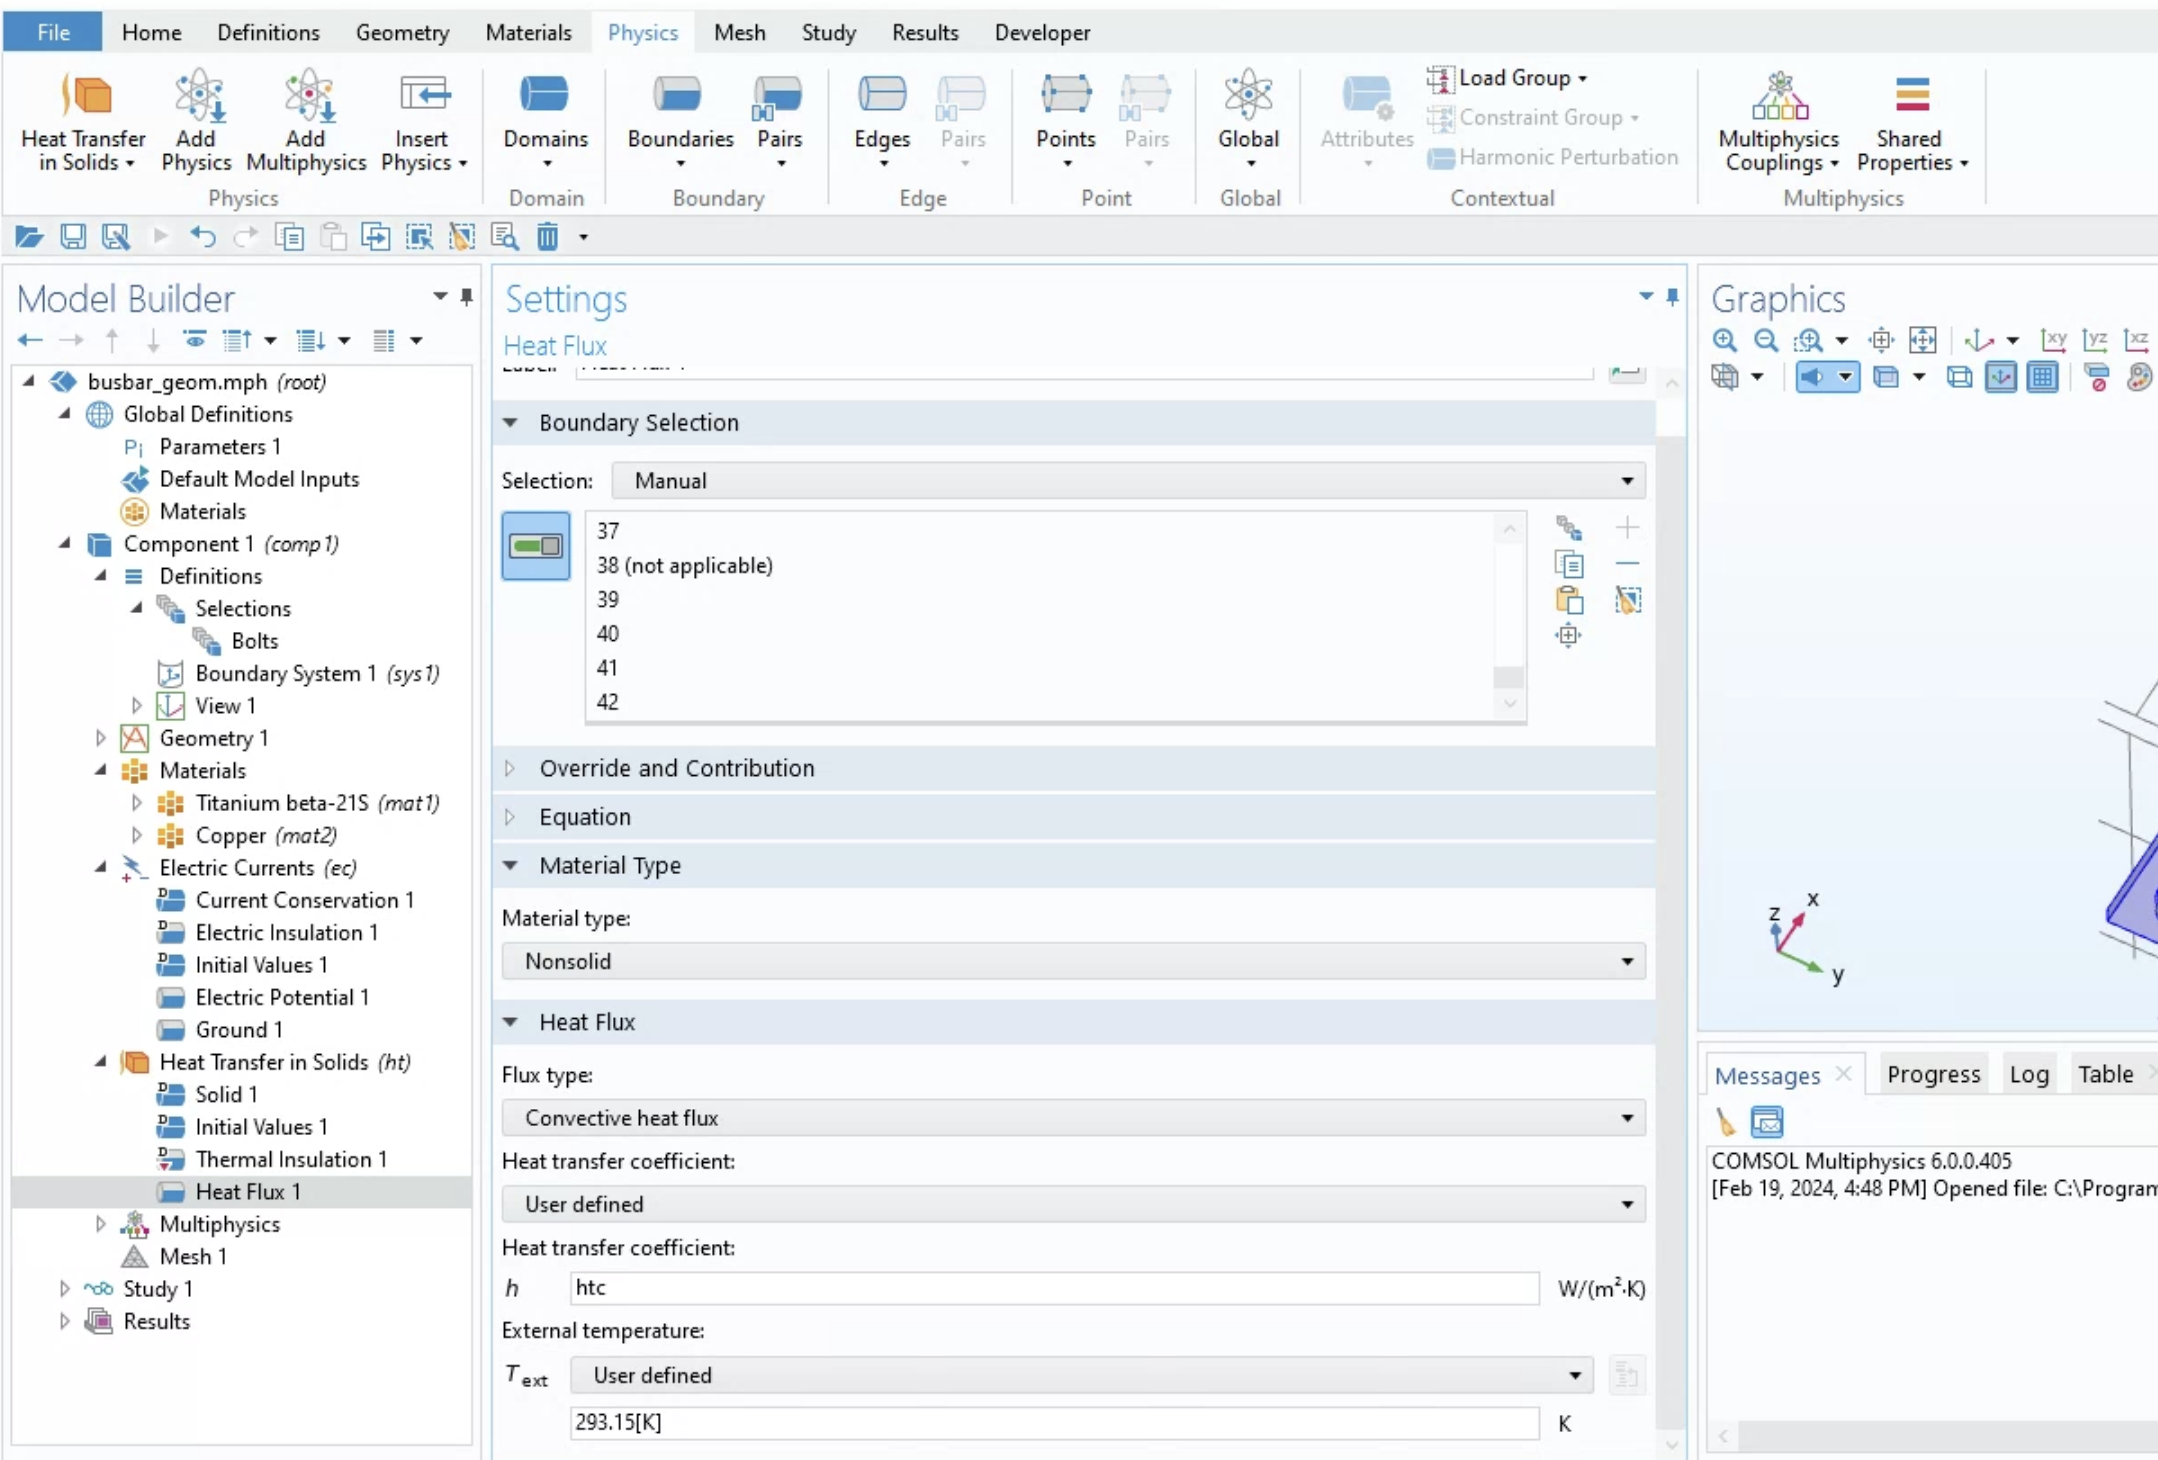
\includegraphics[width=0.4\textwidth]{Chapters/Figures/Chapter 3 Figures/Heat Flux Boundary Conditions.png}
  \caption{Source: \cite{}}
  \label{}
\end{figure}

In this model of a busbar, both of the Physics we've included, Electric Currents and Heat Transfer in solids, are active everywhere.

% SUBSECTION --- Build the Mesh ---
\subsection{Build the Mesh}.
Click the Mesh ribbon tab and select our mesh by clicking the Mesh 1 button. In the Settings window under the Mesh Setting section, if we click the Sequence Type drop-down menu, we have two options. We can always use the default Physics-controlled mesh and this automatically generates a mesh adapted to the Physics settings within the model. The user-controlled mesh allows the user to have manual control over the mesh size and could even create a mesh using different element types.

COMSOL Multiphysics contains different 2D and 3D element types such as pyramids, triangles, prisms among others. COMSOL Multiphysics has nine built-in element size parameter sets, from extremely fine to extremely coarse. To actually build the mesh, we need to click the "Build All" button.

% TODO: Add image showing the mesh of the busbar under "fine"
\begin{figure}[ht!]
  \centering
  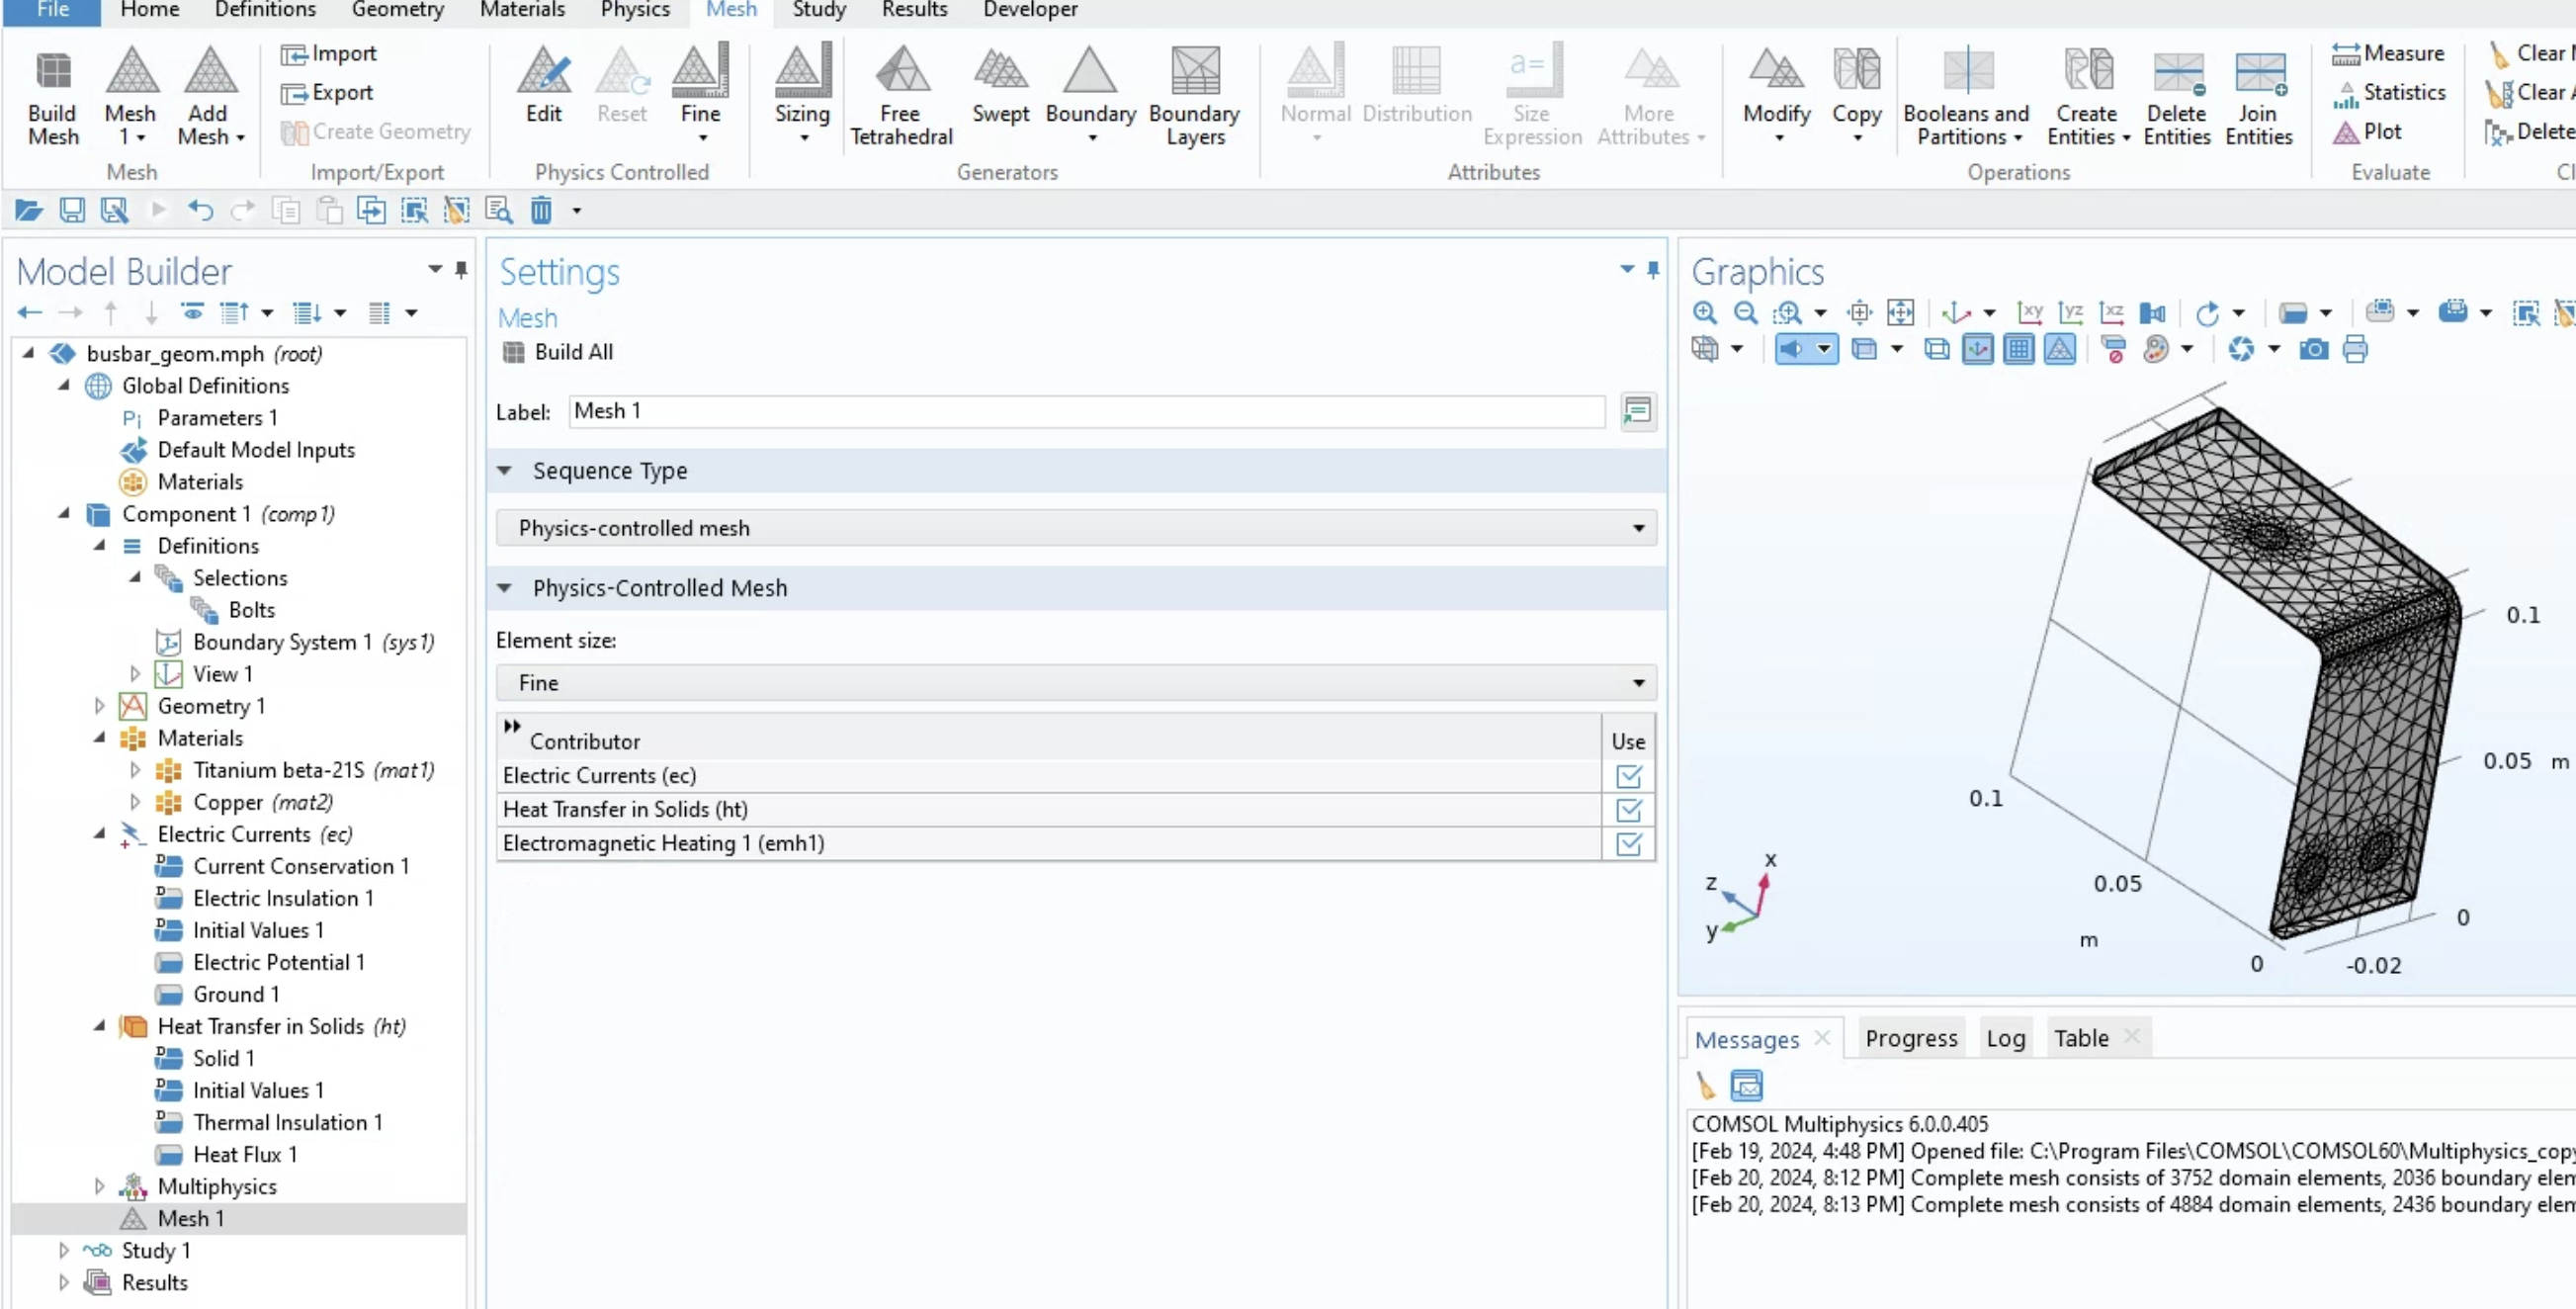
\includegraphics[width=0.4\textwidth]{Chapters/Figures/Chapter 3 Figures/Fine Mesh.png}
  \caption{Source: \cite{}}
  \label{}
\end{figure}

% SUBSECTION --- Run the Study ---
\subsection{Run the Study}.
If we select and expand the Study 1 node, in the Settings window, there's a check box for "Generate default plots" and this will generate plots based on the physics selected in your model. Since our model involves electric currents and heat transfer, we will have results plots including the electric potential as well as the temperature of our busbar.

In the step 1: stationary sub-node under the Physics and Variables dropdown selection, we can see the full multiphysics problem is being computed through the "Solve For Column". We can go ahead and click the "Compute" button. Now that the model has computed, we can move on to the next workflow step and post-process the results.

% TODO: Add image showing computed results.
\begin{figure}[ht!]
  \centering
  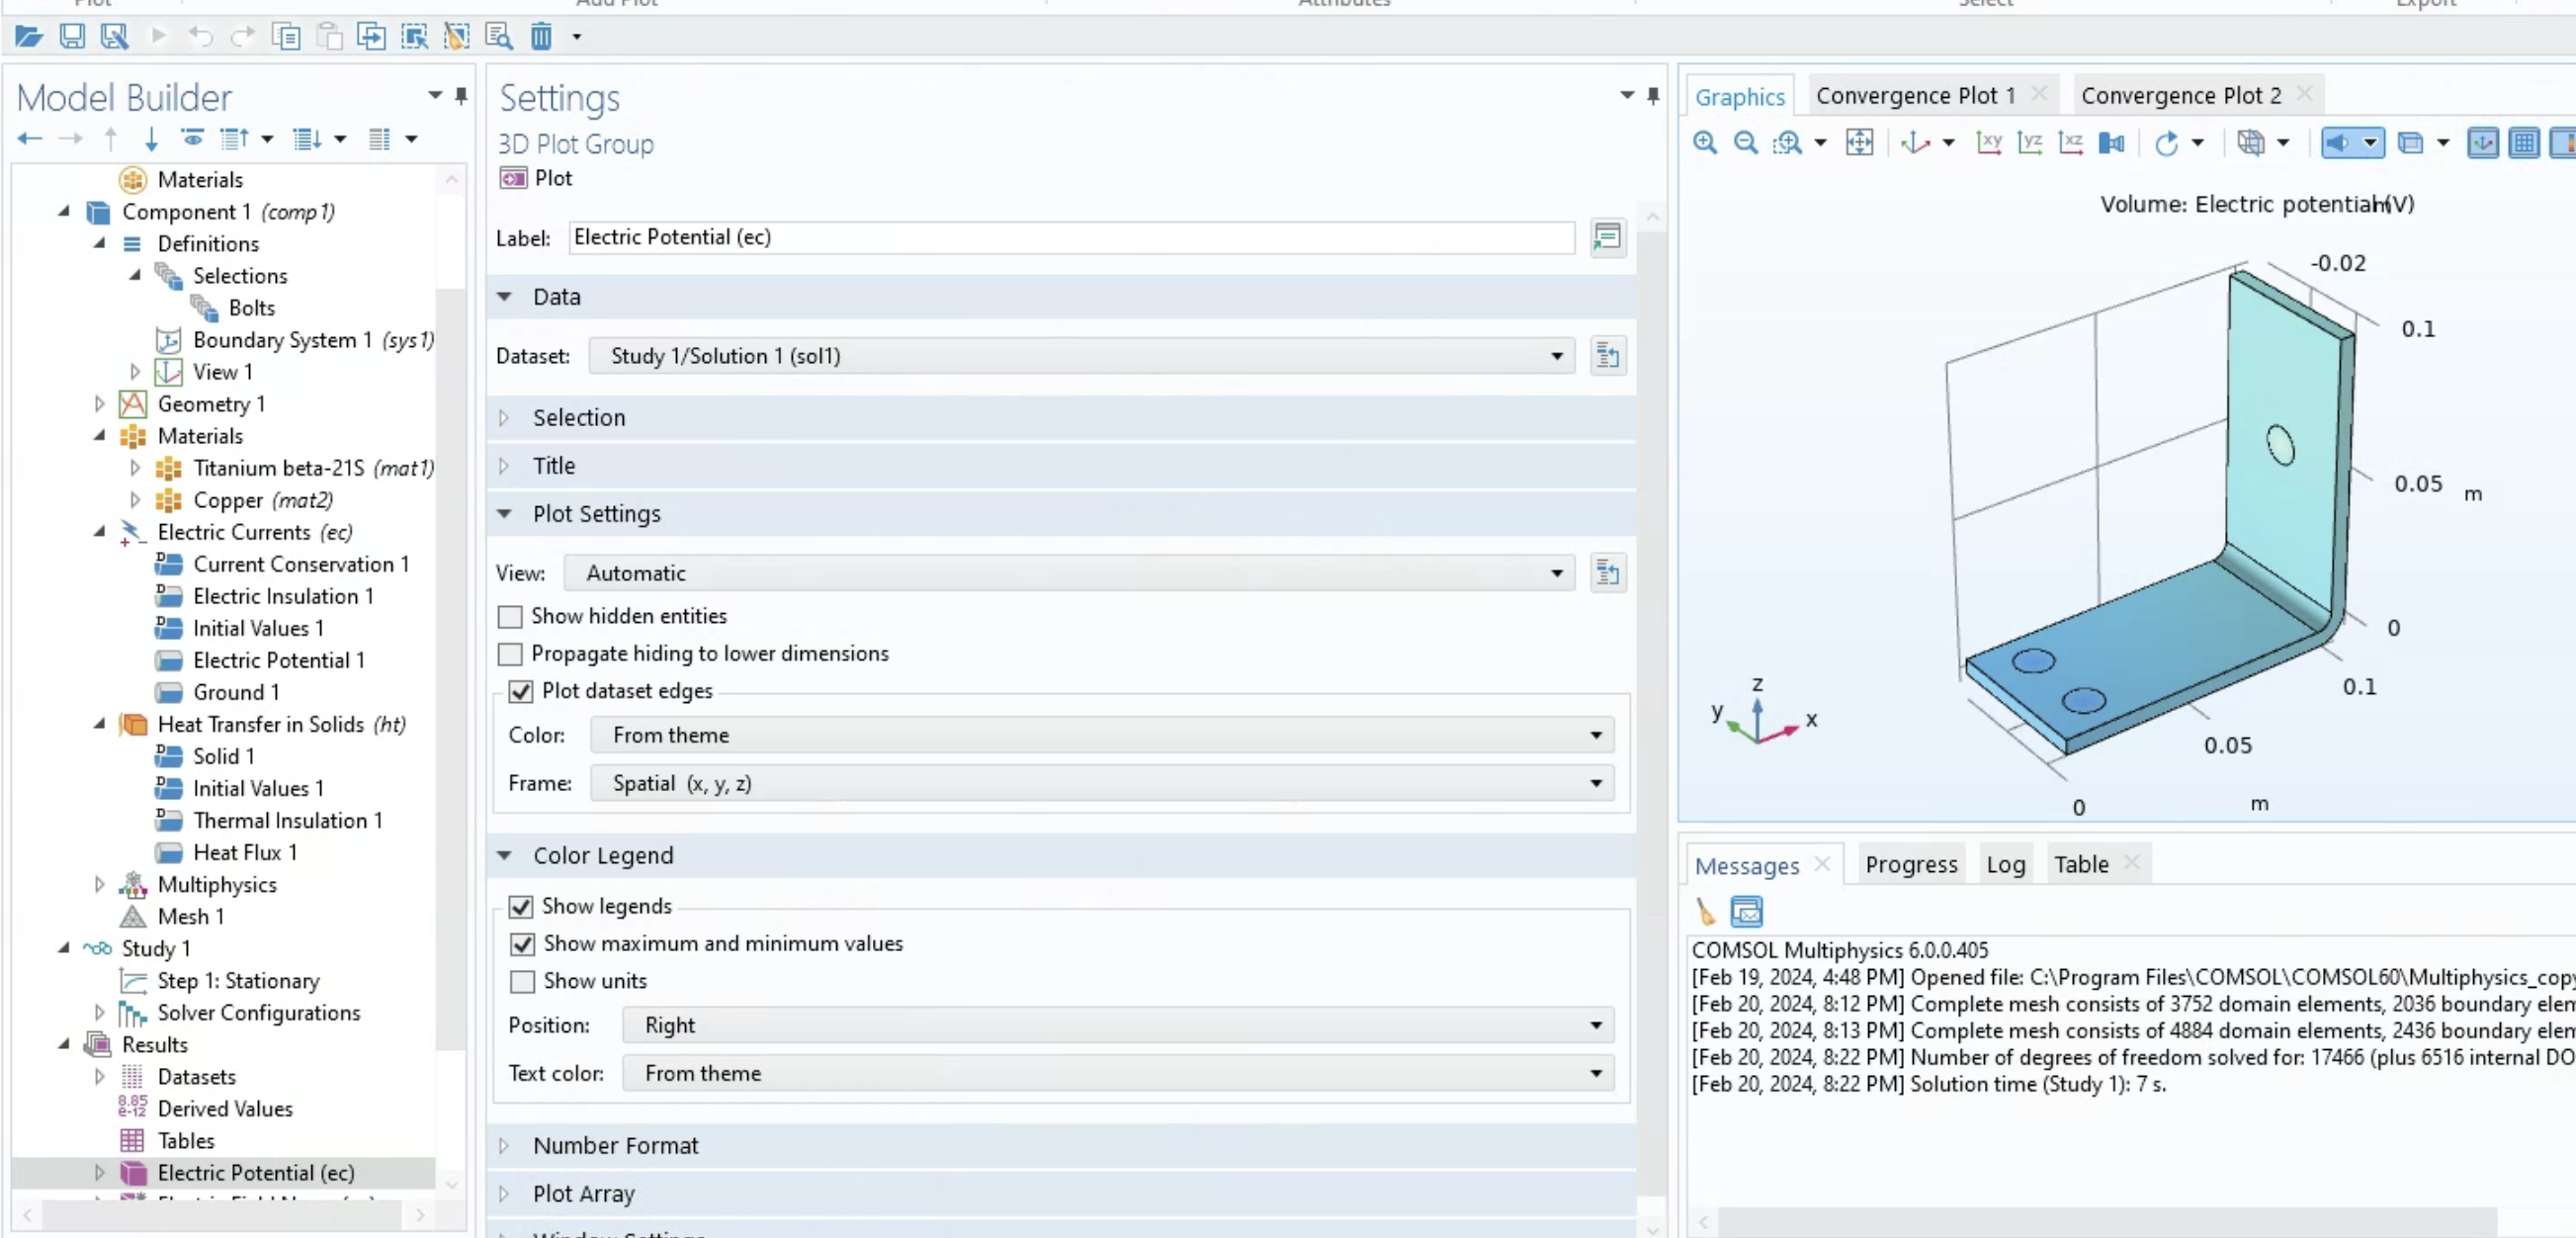
\includegraphics[width=0.4\textwidth]{Chapters/Figures/Chapter 3 Figures/Computed Results.png}
  \caption{Source: \cite{}}
  \label{}
\end{figure}

% SUBSECTION --- Post-Processing the Results ---
\subsection{Post-Processing the Results}.
After completing the workflow to build your model, you can then package it into a simulation app and this is done in the Application Builder. We can create an app from our busbar model that allows us to experiment with the values for some of our parameters.

We can access the Application Builder through the home bar.

% TODO: Add image showing application builder button
\begin{figure}[ht!]
  \centering
  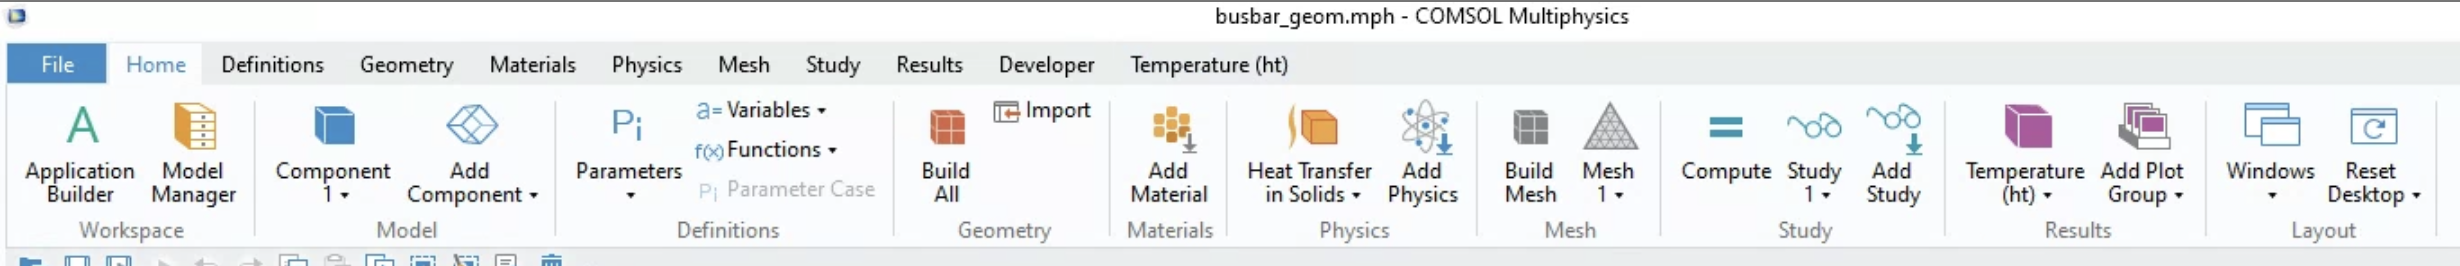
\includegraphics[width=0.4\textwidth]{Chapters/Figures/Chapter 3 Figures/Application Builder Button.png}
  \caption{Source: \cite{}}
  \label{}
\end{figure}

The quick and easy way to create an app is to use the New Form Wizard

% TODO: Add image showing New Form Wizard button
\begin{figure}[ht!]
  \centering
  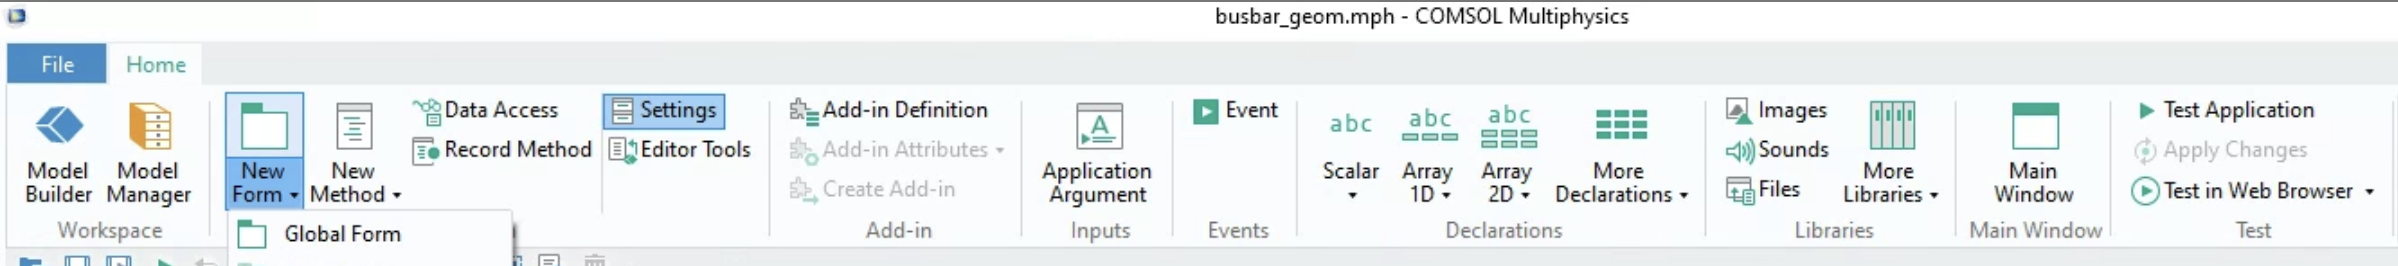
\includegraphics[width=0.4\textwidth]{Chapters/Figures/Chapter 3 Figures/New Form Wizard Button.png}
  \caption{Source: \cite{}}
  \label{}
\end{figure}

We can choose parameters from our model which we can change the values for, and will serve as inputs for our simulation app. For the inputs, we choose the length, width, and applied voltage of the busbar. In the next tab, we can choose the graphics that we want to be available to display in the app. In the next tab, the Buttons tab, we definitely want to include the "Compute Study" button option.

We can click "Done" and this opens the Form Editor and through this we can edit the user interface of our simulation app customizing the appearance, organizing its display using multiple forms, use methods to include additional functionality and much more.

% TODO: Add image showing Form Editor
\begin{figure}[ht!]
  \centering
  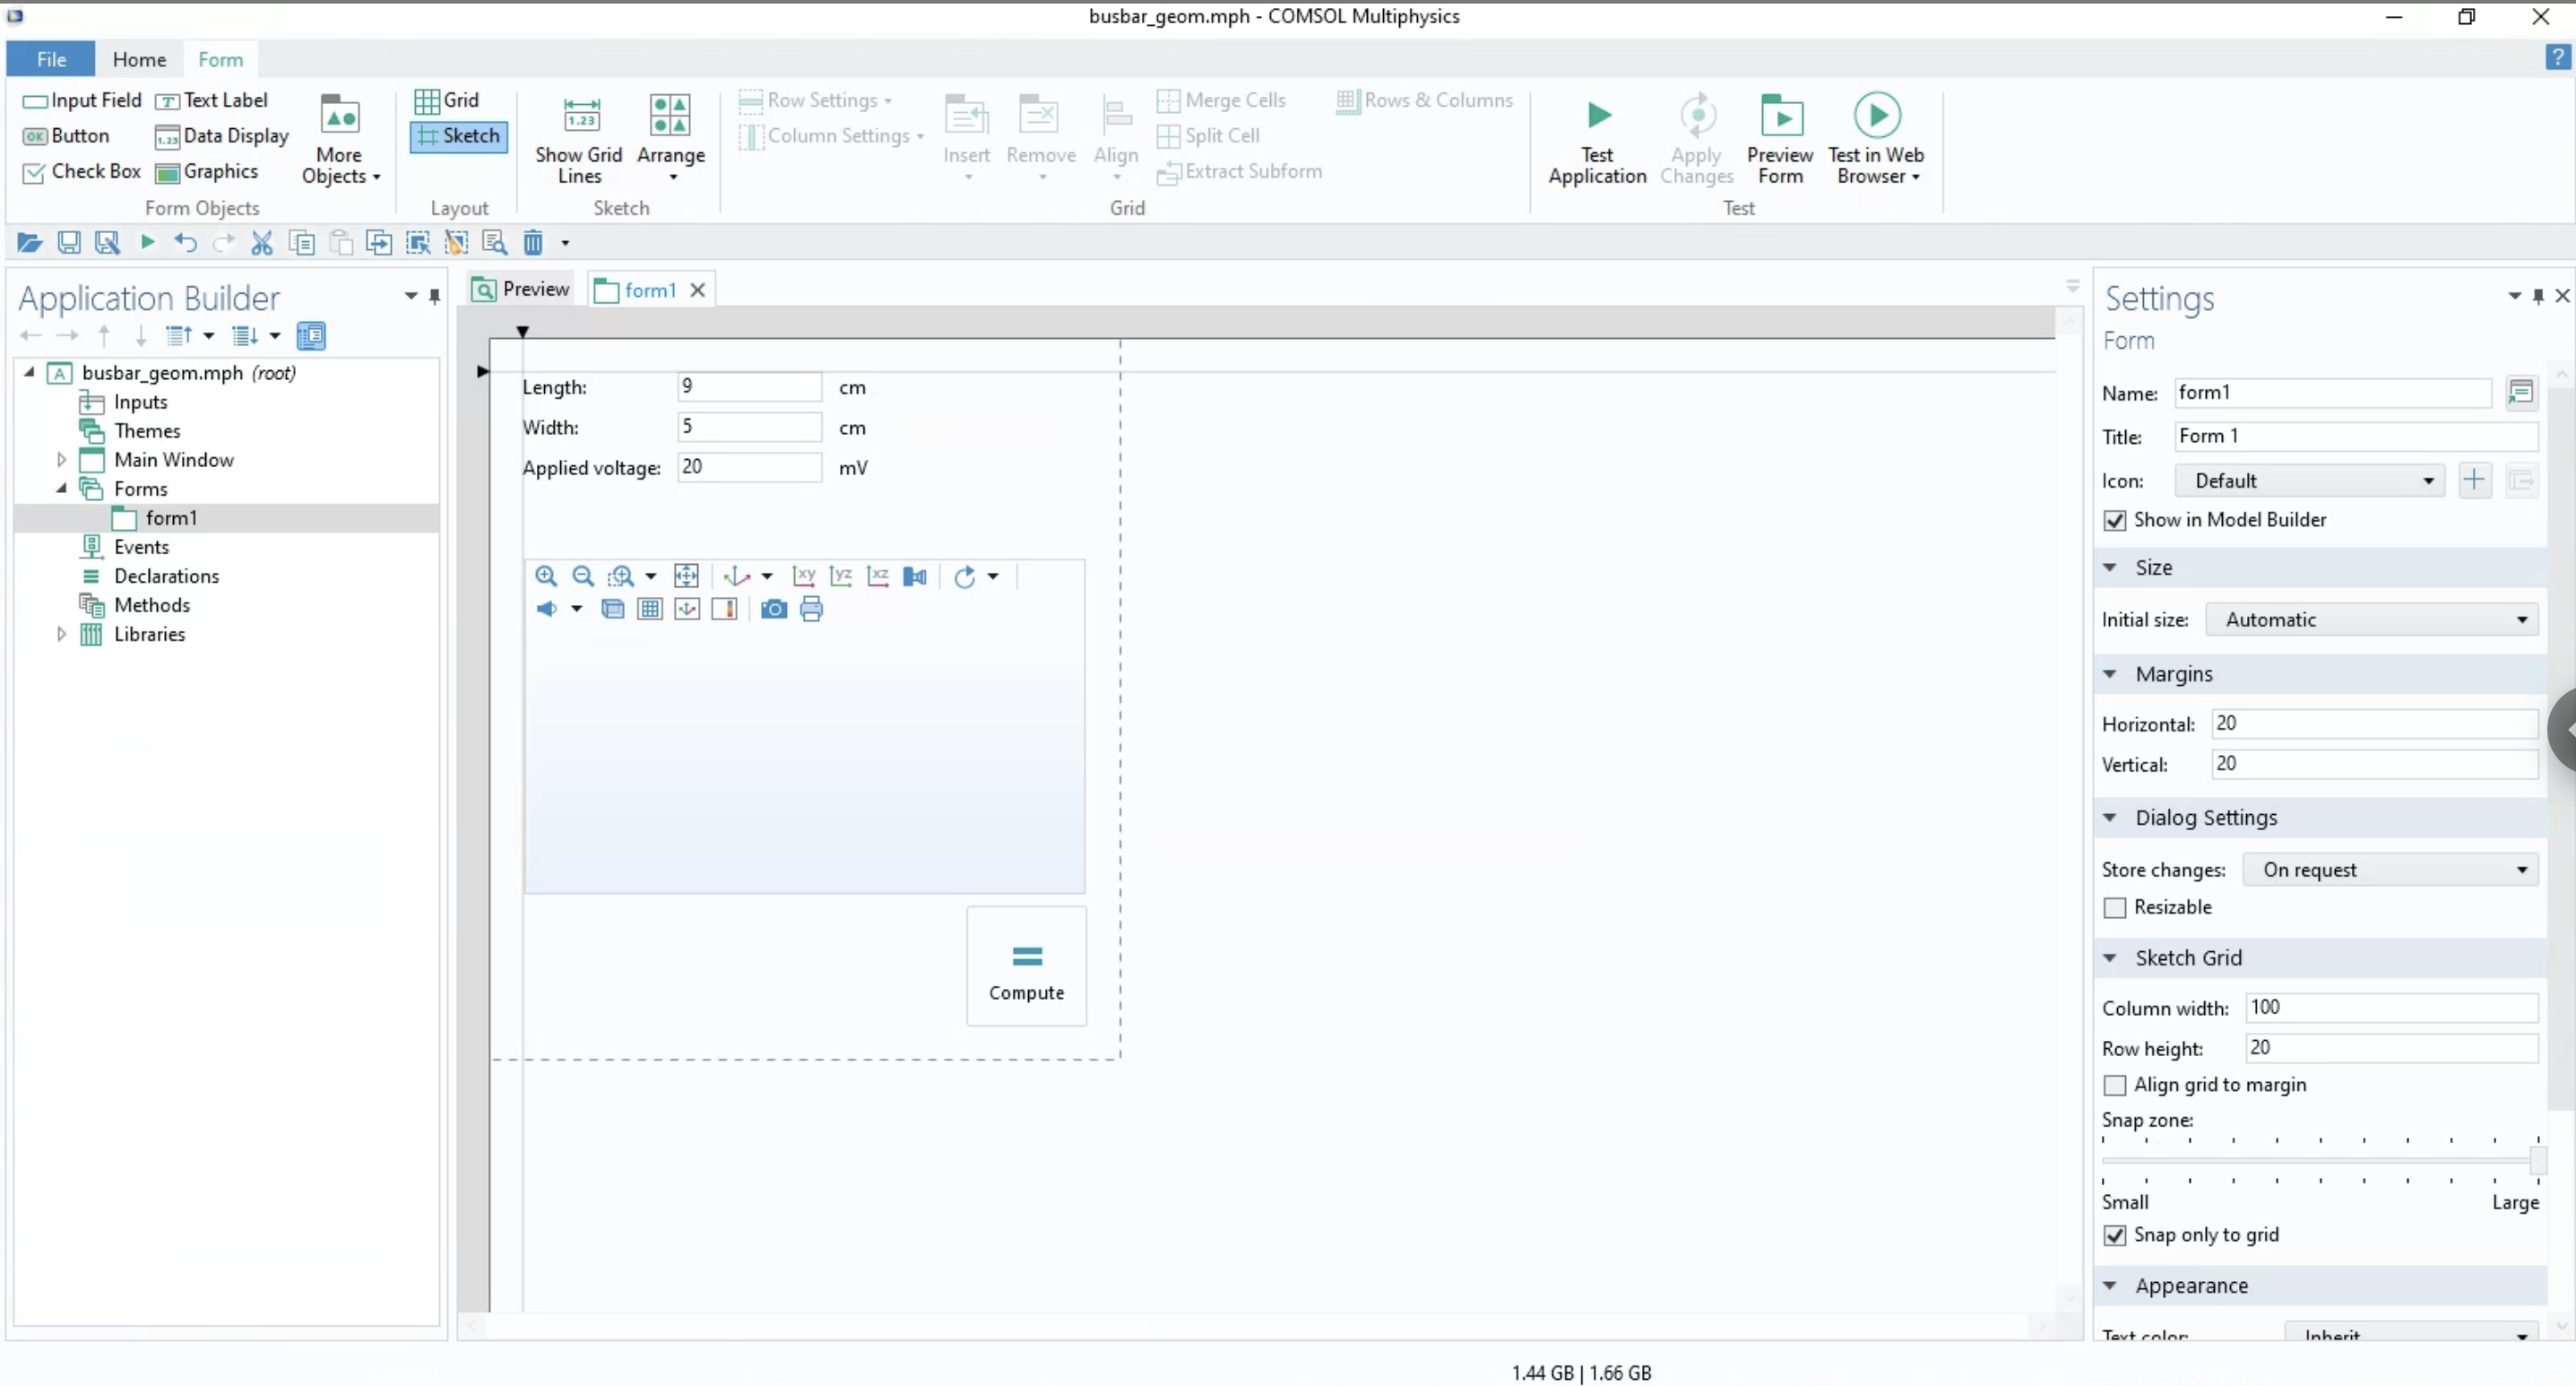
\includegraphics[width=0.4\textwidth]{Chapters/Figures/Chapter 3 Figures/Form Editor Desktop.png}
  \caption{Source: \cite{}}
  \label{}
\end{figure}

If we click the Test Application button, our simulation app appears.

% TODO: Add image after clicking "Test Application" button
\begin{figure}[ht!]
  \centering
  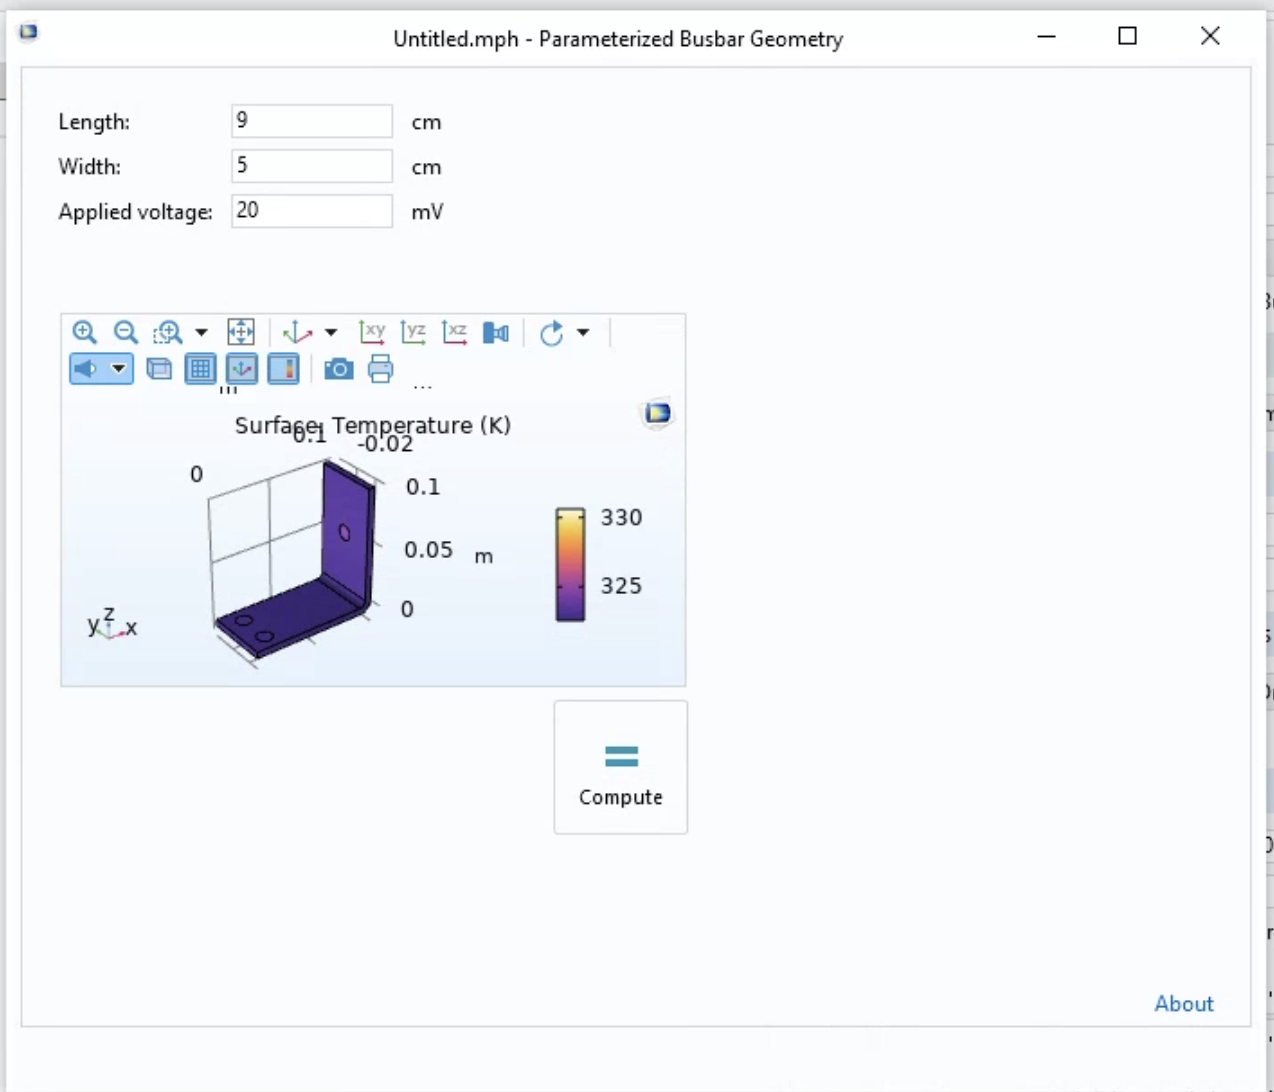
\includegraphics[width=0.4\textwidth]{Chapters/Figures/Chapter 3 Figures/Test Application Results.png}
  \caption{Source: \cite{}}
  \label{}
\end{figure}

We can change some of the values of the parameters such as increasing the length and the width and re-run the app by clicking "Compute".